\documentclass[12pt,a4paper]{article}

\usepackage[onehalfspacing]{setspace}
\usepackage{natbib}
 
\usepackage{float}
%f�r feststellen der figures und tables [H] dranschreiben
\usepackage{siunitx}
%\SI{value}{unit commands} \SI{value}[pre-unit]{unit commands}
%\usepackage{units}
%wird so benutzt: 
%\unit[value/Zahl]{dimension/Einheit} oder 
%\unitfrac[value/Zahl]{dimension/Einheit num/Z�hler}{dimension/Einheit denum/Nenner} oder
%\nicefrac[fontcommand/Schriftart]{dimension/Einheit num/Z�hler}{dimension/Einheit denum/Nenner}
\usepackage{amssymb}
\usepackage{caption}
\usepackage{subcaption}

\usepackage{hyperref}

\usepackage[left=2cm,right=2cm,top=2cm,bottom=2cm]{geometry}
\usepackage[latin9]{inputenc}
\usepackage[ngerman]{babel}
\usepackage[T1]{fontenc}
\usepackage{lmodern}
\usepackage{amsmath}
\usepackage{graphicx}
\usepackage{textcomp}




\begin{document}

%deckblatt erstellen.

\begin{titlepage}

\begin{center}
% Oberer Teil der Titelseite:

\includegraphics[width=0.75\textwidth]{logo.png}\\[1cm]    	%Logo 

\textsc{\LARGE Bergische Universit\"at Wuppertal}\\[1.5cm]	%Institution

\textsc{\Large Fortgeschrittenen Praktikum}\\[0.5cm]				%Projekt


\newcommand{\HRule}{\rule{\linewidth}{0.5mm}}
\HRule \\[0.4cm]
{ \huge \bfseries Rutherford\\ Streuung von $\alpha$-Teilchen}\\[0.4cm]				%Titel

\HRule \\[1.5cm]

% Author und Tutor
\begin{minipage}{0.4\textwidth}
\begin{flushleft} \large
\emph{Verfasser:}\\
Henrik \textsc{J�rgens} \\
Frederik \textsc{Strothmann} \\
\end{flushleft}
\end{minipage}
\hfill
\begin{minipage}{0.4\textwidth}
\begin{flushright} \large
\emph{Tutoren:} \\
Max \textsc{Mustermann} \\
Max \textsc{Mustermann} \\
\end{flushright}
\end{minipage}

\vspace{1cm}

\begin{table}[H]
\centering
\begin{tabular}{|l|}
\hline \textbf{Abstract: } \\
Ziel des Versuches ist es, die Wechselwirkung von $\alpha$-Teilchen mit Materie zu untersuchen.\\
Die Aspekte Streuwinkel, Reichweite, Kernladung und Absorbtionsverhalten werden thematisiert.\\
\hline 
\end{tabular}
\end{table} 

\vspace{1cm}

\begin{table}[H]
\centering
\begin{tabular}{|c|c|c|}
\hline Dies & ist & ein \\ 
\hline Platz- & halter & f�r \\ 
\hline die & bewertungs & Tabelle \\ 
\hline 
\end{tabular} 
\end{table}

\vfill

% Unterer Teil der Seite/Datum
{\large \today}

\end{center}

\end{titlepage}

\newpage
\tableofcontents
\newpage

\bibliographystyle{plain}


\section{Einleitung}
%einleitung zu dem experiment.
%auf die einstellungen, die vor dem versuch gemacht werden, eingehen, oder auf eine anleitung dazu verweisen.
%---------------------------------------------------------------------------------------------
%hinter der einleitung kann der allgemeine theoretische hintergrund in einer zus�tzlichen section erkl�rt werden
In diesem Versuch werden Oberfl�chen verschiedener Proben mittels Rasttunnelmikroskopie auf deren Gitterstruktur und morphologische Eigenschaften untersucht. Elektronendichte, Oberfl�chenrauheit und die atomare Gitterstruktur k�nnen mit dem Rastertunnelmikroskop (RTM) analysiert werden. Der quantenmechanische Tunneleffekt wird genutzt, um leitende Materialien zu untersuchen. Indem zwischen einer einatomigen Platin-Iridum-Elektrode und der zu untersuchenden Probe eine Potentialdifferenz angelegt wird, kommt es abh�ngig von der Entfernung der Pt-Ir-Elektrode zur Probe und dessen Elektronendichte zu einem Tunnelstrom, welcher R�ckschl�sse auf die Struktur der Probe erlaubt. Die Elektronendichte der Oberfl�che kann durch systematisches Abrastern der Probe erfasst werden, sodass mithilfe verschiedener Modi (CC und CH: Constant Current und Constant Height) ein Bild der Materialoberfl�che entsteht.
\section{Theorie}
% Es sollen die wichtigsten theoretischen Formeln und Zusammenh�nge einmal ausf�hrlich erkl�rt werden
Es werden die theoretischen Grundlagen zur Bestimmung der Lebensdauer von Myonen besprochen.

\subsection{Standardmodell}
Das Standartmodell der Teilchenphysik drei der vier Grundlegenden Wechselwirkungen (WW), die schwache WW, die elektromagnetische WW und die Starke WW.
Die Kr�fte wechselwirken �ber Vektorbosonen, welche eine ganzzahligen Spin haben.
In Tabelle \ref{tab:ww} ist eine �bersicht der drei Kr�fte zu sehen.

\begin{table}[H]
\caption{In der Tabelle sind die Grundlegenden WW (au�er der Gravitation) und ihre Eigenschaften aufgetragen (entnommen \cite{povh} Seite 274)}
\label{tab:ww}
\centering
\begin{tabular}{|c|c|c|c|c|}
\hline Wechselwirkung & koppelt an & Austauschteilchen & $\frac{m_0}{GeV}$ & J$^P$ \\ 
\hline stark & Farbe & 8 Gluonen (g) & 0 & 1$^-$ \\ 
\hline elektromagnetisch & elektrische Ladung & Photon ($\gamma$) & 0 & 1$^-$ \\ 
\hline schwach & schwache Ladung & W$^\pm$, Z$^0$ & $\approx 10^2$ & 1 \\ 
\hline 
\end{tabular} 
\end{table}
Neben den Bosonen gibt es noch zwei weitere Fundamentale Teilchenarten die Quark und die Leptonen welche die Grundbausteine der Materie darstellen.
Beide geh�ren zu den Fermionen, haben also einen halbzahligen Spin. Leptonen und Quarks werden mit aufsteigender Masse in drei Generationen aufgeteilt.
In Tabelle \ref{tab:fermi} sind Quarks und Leptonen mit ihren Eigenschaften dargestellt.

\begin{table}[H]
\caption{�bersicht der Grundlegenden Eigenschaften von Quarks und Leptonen}
\label{tab:fermi}
\centering
\begin{tabular}{|p{2cm}|p{2cm}|p{2cm}|p{1cm}|p{3.5cm}|p{1cm}|}
	\hline
	Fermionen & \hspace{0.25cm} Familie \newline 1 \hspace{0.3cm} 2 \hspace{0.3cm} 3                                               & elektrische Ladung    & Farbe  & schwacher Isospin \newline rechtsh. \hspace{0.5cm} linksh. & Spin \\ \hline
	Leptonen  & $\nu_e$ \hspace{0.17cm} $\nu_\mu$ \hspace{0.17cm} $\nu_\tau$ \newline e \hspace{0.3cm} $\mu$ \hspace{0.3cm} $\tau$ & \hspace{0.6cm} 0 \newline  \hspace*{0.6cm} -1      & ------ & 1/2 \hspace{1.5cm} --- \newline \hspace*{2.4cm} 0          & 1/2  \\ \hline
	Quarks    & u \hspace{0.3cm} c \hspace{0.3cm} t \newline d \hspace{0.3cm} s \hspace{0.3cm} b                                   & \hspace*{0.2cm} +2/3 \newline \hspace*{0.3cm} -1/3 & r,g,b  & 1/2 \hspace{1.64cm} 0 \newline \hspace*{2.4cm} 0           & 1/2  \\ \hline
\end{tabular} 
\end{table}


\section{Versuchsaufbau}
%skizze zum versuchsaufbau (oder foto) einf�gen,   es muss erkl�rt werden wie das ganze funktioniert und welche speziellen einstellungen verwendet wurden (z.b. welche kn�pfe an den ger�ten f�r die messung verdreht wurden)
F�r den Versuch werden zwei verscheiden Vakuumkammern verwendet. Die erste Kammer  ist eine Rutherford-Streukammer, eine schematische Skizze ist in Abb. \ref{fig:kammer} zu sehen. Die Streukammer besteht aus einer Vakuumkammer, mit durchsichtigem Deckel. Ein Barometer, ein Bel�ftungsventil und ein Ventil mit Anschluss an die Vakuumpumpe sind an den Absperrhahn (3) angeschlossen. Der Halbleiterdetektor mit Kollimator (12,12.1) ist von innen an einer BNC-Buchse (2.1) montiert. Von au�en ist ein Vorverst�rker angeschlossen, die Daten werden von einem Digitalz�hler, der an einen Computer angeschlossen ist ausgelesen (siehe Abb. \ref{fig:aufbau}). Der Deckel der Streukammer hat einen Schwenkarm (7), an dem das $^{241}$Am-Pr�parat (7.1) , verschiedene Rahmen mit SpaltkKollimatoren (9) und Metallfolien (10) angebracht werden k�nnen. �ber einen Knopf (4) ist der Schwenkarm drehbar, der Winkel ist dabei �ber eine Skala (8) ablesbar. Zur Verf�gung stehen Spalte mit 1m und 5mm Breite sowie eine Goldfolie mit 2$\mu$m und eine Aluiminiumfolie mit 7$\mu$m Dicke.

\begin{figure}[H]
	\centering
  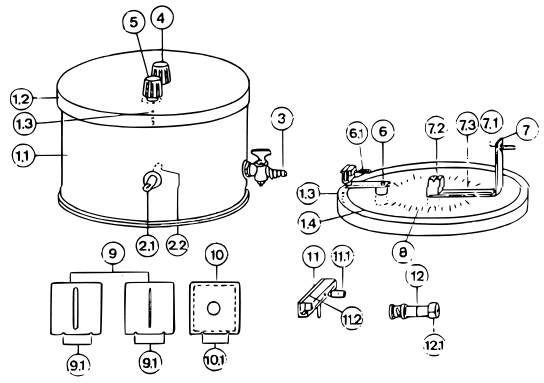
\includegraphics[scale=0.4]{streukammer.png}
	\caption{Schematischer Aufbau des Streukammer}
	\label{fig:kammer}
\end{figure}


\begin{figure}[H]
	\centering
  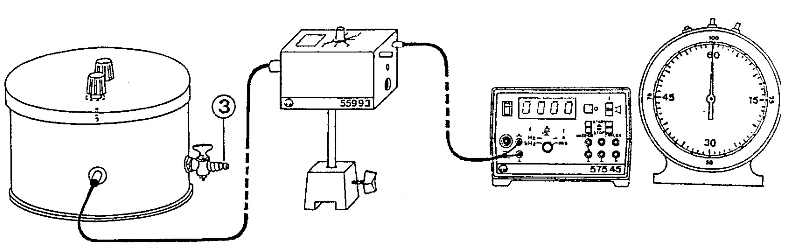
\includegraphics[scale=0.4]{aufbau.png}
	\caption{Schematischer Aufbau des Versuchsaufbaus}
	\label{fig:aufbau}
\end{figure}

Die zweite Kammer ist eine Vakuumkammer, mit einer optischen Bank, zu befestigen der radioaktiven Quelle. Sie wird f�r die Bestimmung der Reichweite von $\alpha$-Strahlung und die Untersuchung von Absorbtion durch verschiedenen Medien verwendet. Der Detektor ist an einen PC angeschlossen mit dem die Messdaten aufgenommen werden.
\section{Rutherford-Streuversuch}
%kurz das ziel dieses versuchsteiles ansprechen, damit keine zwei �berschriften direkt �bereinander stehen!
%bei schwierigeren versuchen kann auch der theoretische hintergrund erl�utert werden. (mit formeln, herleitungen und erkl�rungen)
In diesem Versuchsabschnitt soll die Streuung von $\alpha$-Strahlung an Goldfolie untersucht werden.

\subsection{Versuchsdurchf�hrung}
Die Streuung von $\alpha$-Teilchen an einer Goldfolie wird in einem Winkelbereich von -30$^\circ$ bis 30$^\circ$ in 5$^\circ$-Schritten untersucht. Neben der Goldfolie wird der Kollimator mit einer Spaltbreite von 1mm eingesetzt. Die Streukammer wird auf 35 mbar evakuiert. Die Messdaten werden mit dem Computer aufgenommen. F�r jeden Winkel wurde f�r einen Zeitraum von 3min gemessen. Die aufgenommen Histogramme werden mit der Poissonverteilung gefittet (Beispiel im Anhang). Der Fehler des Winkels wurde mit 2$^\circ$ angenommen. Die so Bestimmten Z�hlraten werden mit Gl. \ref{eqn:ruth} gefittet. Da das Winkelma� einen Offset besitzt, wird dies durch eine additive Konstante als Fitparameter ber�cksichtigt.

\begin{align}
\label{eqn:ruth}
f(x) = \frac{A}{sin^4 \left[ \frac{\pi (x-B)}{180} \right]}
\end{align}

\subsection{Auswertung}
In Abb. \ref{fig:rutherford_gold} sind die Messdaten mit dem Fit der Rutherfordstreuformel zu sehen. Die Rutherfordstreuuformel wurde nach GL. \ref{eqn:ruth} gefittet. Dabei ergaben sich f�r den Fit die Werte in Tabelle \ref{tab:fit_gold_ruth}.

\begin{figure}[H]
	\centering
  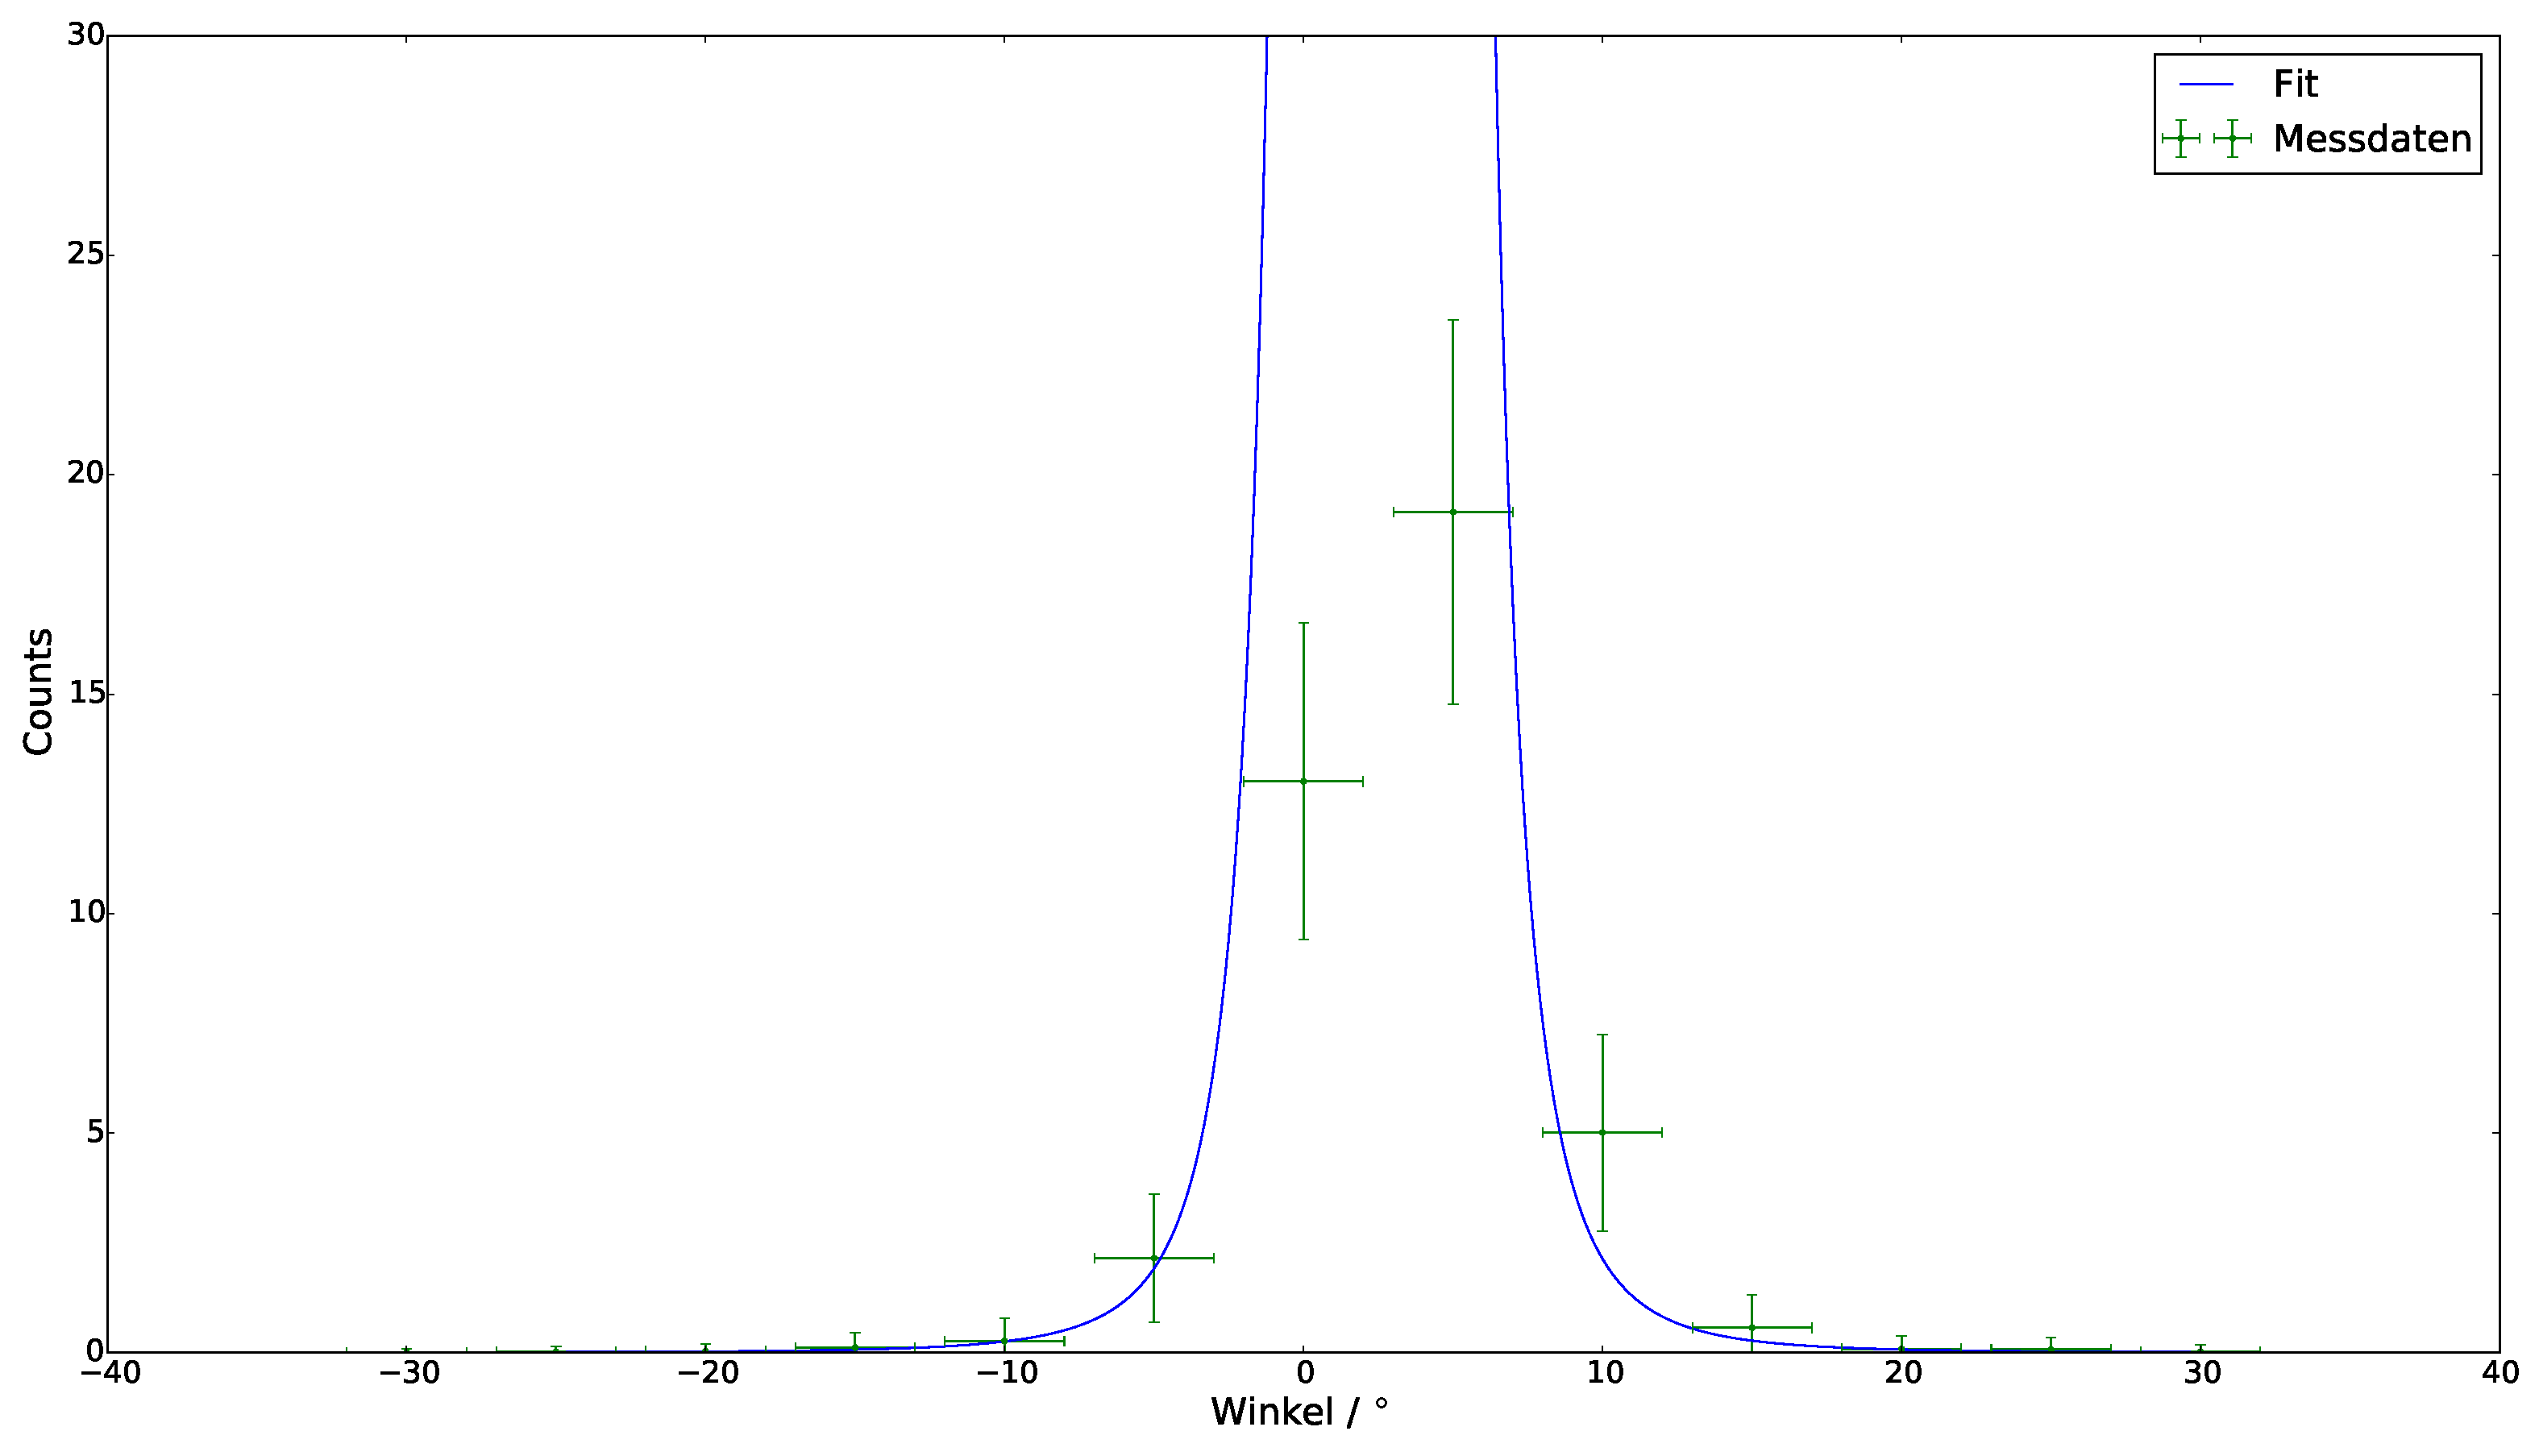
\includegraphics[scale=0.33]{rutherford_messung.pdf}
	\caption{Es sind die Messdaten aus der Streuung von $\alpha$-Strahlung an Gold zu sehen. Die Messdaten wurden mit  Gl. \ref{eqn:ruth} gefittet, dabei ergab sich ein $\chi_{red}^2$ von 2,48.}
	\label{fig:rutherford_gold}
\end{figure}

\begin{table}[H]
\centering
\caption{Fitparamter f�r die Goldfolie nach Gl. \ref{eqn:ruth}}
\label{tab:fit_gold_ruth}
\begin{tabular}{|c|c|}
\hline Paramter & Wert \\ 
\hline A & 0,00037 $\pm$ 0,00002 \\ 
\hline B & 2,62 $\pm$ 0,05 \\ 
\hline $\chi_{red}^2$ & 2,48 \\ 
\hline 
\end{tabular} 
\end{table}


Der Fit passt optisch gut zu den Daten, auch wenn das $\chi_{red}^2$ nur einen Wert von 2,48 hat.
\section{R�ckstreuung von $\alpha$-Teilchen}
%kurz das ziel dieses versuchsteiles ansprechen, damit keine zwei �berschriften direkt �bereinander stehen!
%bei schwierigeren versuchen kann auch der theoretische hintergrund erl�utert werden. (mit formeln, herleitungen und erkl�rungen)
Es soll qualitativ die R�ckstreuung von $\alpha$-Teilchen untersucht werden. Mit dem zuvor bestimmten Fit kann der Wert f�r einen Winkel von 150$^\circ$ bestimmt werden.

\subsection{Versuchsdurchf�hrung}
Die Goldfolie wird ohne Spalt in die Kammer eingesetzt und ein Winkel von 150$^\circ$ eingestellt. Da eine sehr geringe Z�hlrate erwartet wird, wird �ber einen Zeitraum von einer Stunde gemessen.

\subsection{Auswertung}

�ber den Zeitraum von 60 Minuten wurden 5 Counts gemessen, dies entspriche einer Rate von 0.0014 Counts/s. Die niedrige Z�hlrate zeigt, das die Rutherfordstreuuformel f�r gro�e Winkel nicht mehr zutrifft.
\section{Bestimmung der Kernladungszahl von Aluminium}
%kurz das ziel dieses versuchsteiles ansprechen, damit keine zwei �berschriften direkt �bereinander stehen!
%bei schwierigeren versuchen kann auch der theoretische hintergrund erl�utert werden. (mit formeln, herleitungen und erkl�rungen)
Es soll die Kernladungszahl von Aluminium bestimmt werden. Die Winkelverteilung der Z�hlraten soll mit denen der Goldfolie verglichen werden.

\subsection{Versuchsdurchf�hrung}
Die Aluminiumfolie und der 1mm Spalt werden eingesetzt. Dann werden die Z�hlraten f�r verschiedene Winkel �ber einen Zeitraum von ??s aufgenommen.

\subsection{Auswertung}
Die Kernladungszahl wird mit zwei verschiedenen Methoden bestimmt. In der ersten Methode wird die Rutherfordstreuuformel (Gl. ??) an die Z�hlraten gefittet. Dabei entspricht der Parameter Z$_2$ der Kernladungszahl von Aluminium. Die Messdaten mit dem Fit sind in Abb. ?? zu sehen. F�r den Fit ergaben sich die Werte in Tabelle ??.


F�r die zweite Methode wird Gl. ?? verwendet, dabei werden f�r die festen Parameter die Werte in Tabelle ?? verwendet.

\begin{table}[H]
\centering
\caption{Werte der festen Parameter f�r die Bestimmung der Kernladungszahl von Aluminium nach Gleichung ??}
\label{tab:alu_paras}
\begin{tabular}{|c|c|}
\hline Parameter & Wert \\ 
\hline $Z^2_{Au}$ & 79 \\ 
\hline $d_{Au}$ & 2 [$\mu$m] \\ 
\hline $d_{Al}$ & 7 [$\mu$m] \\ 
\hline \.{N}$_{Au}$ &  \\ 
\hline \.{N}$_{Al}$ &  \\ 
\hline 
\end{tabular} 
\end{table}
\section{Reichweitenbestimmung}
%kurz das ziel dieses versuchsteiles ansprechen, damit keine zwei �berschriften direkt �bereinander stehen!
%bei schwierigeren versuchen kann auch der theoretische hintergrund erl�utert werden. (mit formeln, herleitungen und erkl�rungen)
Es soll die Reichweite von $\alpha$-Strahlung bei Normaldruck untersucht werden.

\subsection{Versuchsdurchf�hrung}
Es werden keine Metallfolien oder Kollimationsspalte verwendet. Der Schwenkarm wird auf 0$^\circ$ eingestellt. Da der Abstand zwischen Dem $^{241}$Am-Pr�parat und der Quelle nicht ver�nderbar ist, kann die Abstandsabh�ngigkeit nicht direkt bestimmt werden. Stattdessen wird die Z�hlrate in Abh�ngigkeit des Luftdrucks aufgenommen. Da die Reichweite linear mit Anzahl der St��e mit den Luftmolek�len abh�ngt, h�ngt die Reichweite unter Annahme des idealen Gassesetztes auch linear von Druck ab. Daraus l�sst sich f�r die Reichweite unter Normaldruck Gl. \ref{eqn:reich_normal} folgern.

\begin{align}
\label{eqn:reich_normal}
x_{Normal} = x_{Messung} \frac{p_{Messung}}{p_{Normal}} 
\end{align}

Der Druck wird solange in Schritten von ?? erh�ht, bis die Countrate auf 0 abf�llt. Mit dem Zusammenhang, aus Gl. \ref{eqn:reich_normal} kann die Reichweite von $\alpha$-Strahlung in Luft bestimmt werden.

\subsection{Auswertung}

\section{Energieverlust von $\alpha$-Strahlung in Luft}
%kurz das ziel dieses versuchsteiles ansprechen, damit keine zwei �berschriften direkt �bereinander stehen!
%bei schwierigeren versuchen kann auch der theoretische hintergrund erl�utert werden. (mit formeln, herleitungen und erkl�rungen)
\label{sec:energieverlust}
In diesem Versuchsabschnitt soll der Energieverlust von $\alpha$-Strahlung in Luft, bei Normaldruck, untersucht werden.


\subsection{Kanal-Energie-Eichung}
Dann wird eine Kanal-Zeit-Eichung mit der Zerfallsreihe von $^{266}$Ra durchgef�hrt. Die Zerfallsreihe ist in Abb. \ref{fig:zerfall} zu sehen. Die Peaks werden �ber einen Multi-Gauss-Fit bestimmt. Der 5,49 MeV und der 5,30 MeV Peak liegen so nah bei einander, dass er von dem Detektor nicht aufgel�st werden kann, deshalb, werde bei dem als ein Peak interpretiert. Dieser besteht aus einer Summe von 4 Gaussverteilungen. Den so bestimmten Kan�len kann mit der Zerfallskette (Abb. \ref{fig:zerfall}) eine Energie zugeordnet werden. Die Werte werden mit einer linearen Funktion gefittet (Gleichung \ref{eqn:lin}).


\begin{figure}[H]
	\centering
  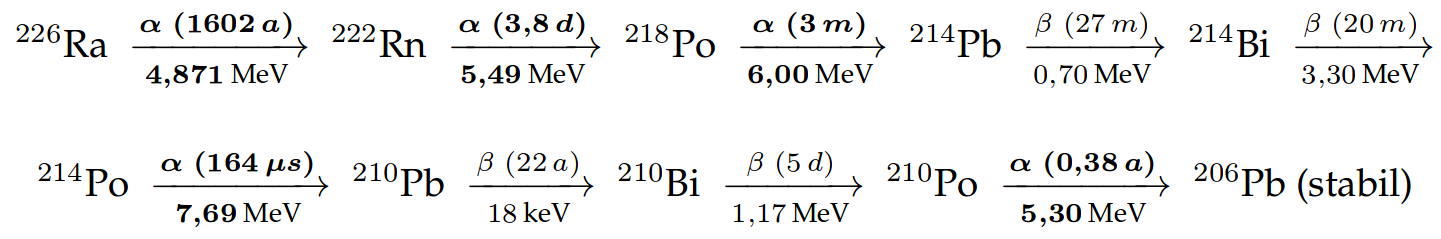
\includegraphics[scale=0.33]{zerfalls_reihe.png}
	\caption{Zerfallsreihe von $^{266}$Ra. Entnommen aus \cite{anleitung}}
	\label{fig:zerfall}
\end{figure}


\begin{align}
\label{eqn:lin}
E(k) = A \cdot k + B
\end{align}

Da nur Fehler auf den Kanal vorhanden sind, wird Gleichung \ref{eqn:lin} zu Gleichung \ref{eqn:lin_neu} umgeformt und damit die Fehler im Fit zu ber�cksichtigen.

\begin{align}
\label{eqn:lin_neu}
k = \frac{E-B}{A}
\end{align}

Der Multi-Gauss-Fit ist in Abbilung \ref{fig:multi_fit} zu sehen. Dabei ergaben sich die Fitparameter in Tabelle \ref{tab:multi-fit}. Die Kurve passt optisch gut zu den Messdaten, was durch ein reduziertes Chiquadrat $\chi_{red}^2$ von 1,717 best�tigt wird.

\begin{figure}[H]
	\centering
  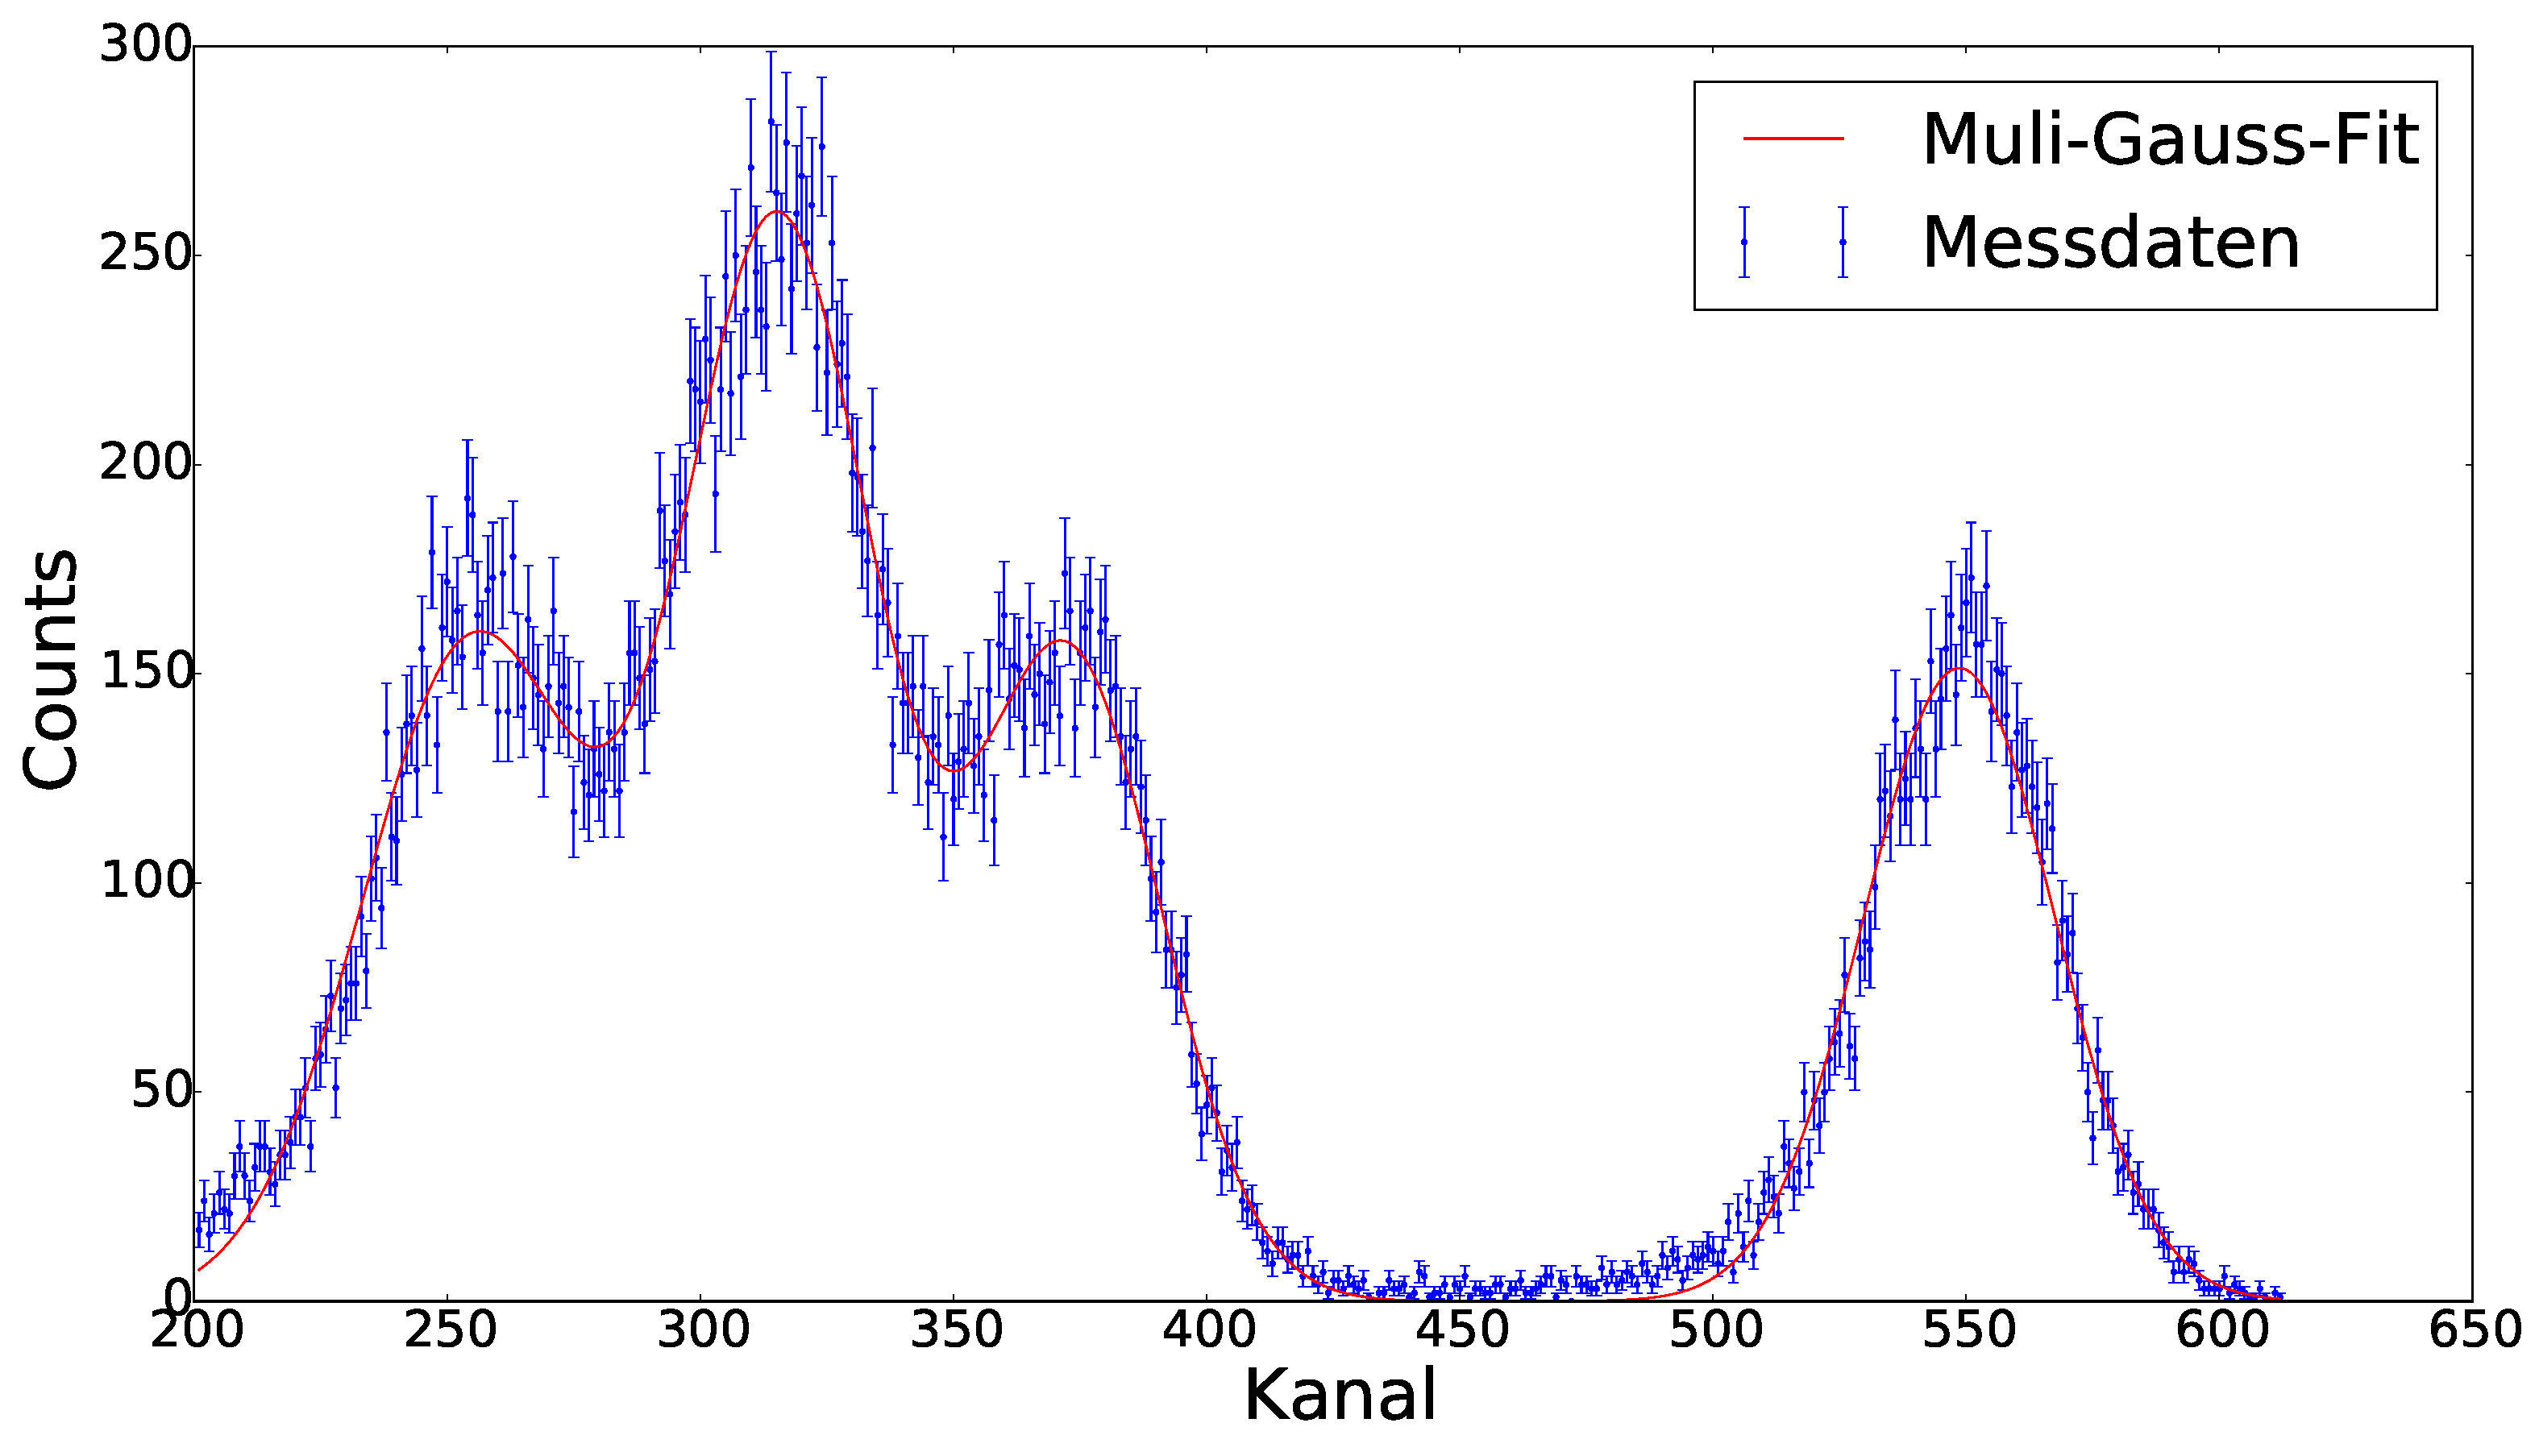
\includegraphics[scale=0.33]{multi_fit.pdf}
	\caption{Messung des $^{226}$Ra-Zerfalls mit Multi-Gauss-Fit}
	\label{fig:multi_fit}
\end{figure}


\begin{table}[H]
\centering
\caption{$\mu$-Parameter des Multi-Gauss-Fits}
\label{tab:multi-fit}
\begin{tabular}{|c|c|c|}
\hline Gausskurve & Wert & Fehler \\ \hline
\hline 1  & 255,0 & 1,0 \\ 
\hline 2  & 315,5 & 0,6 \\ 
\hline 3  & 372,5 & 0,8 \\ 
\hline 4  & 548,6 & 0,3 \\ 
\hline 
\end{tabular} 
\end{table}

Mit den bestimmten Kan�len und den Energien ergibt sich der Plot in Abb. \ref{fig:linear_fit}. Die Ergebnisse des Fits sind in Tabelle \ref{tab:linear-fit} aufgetragen. Das reduzierte Chiquadrat $\chi_{red}^2$ hat einen Wert von 3.01. Die Energie eines Kanals ist durch Gleichung \ref{eqn:energie-kanal} gegeben.

\begin{figure}[H]
	\centering
  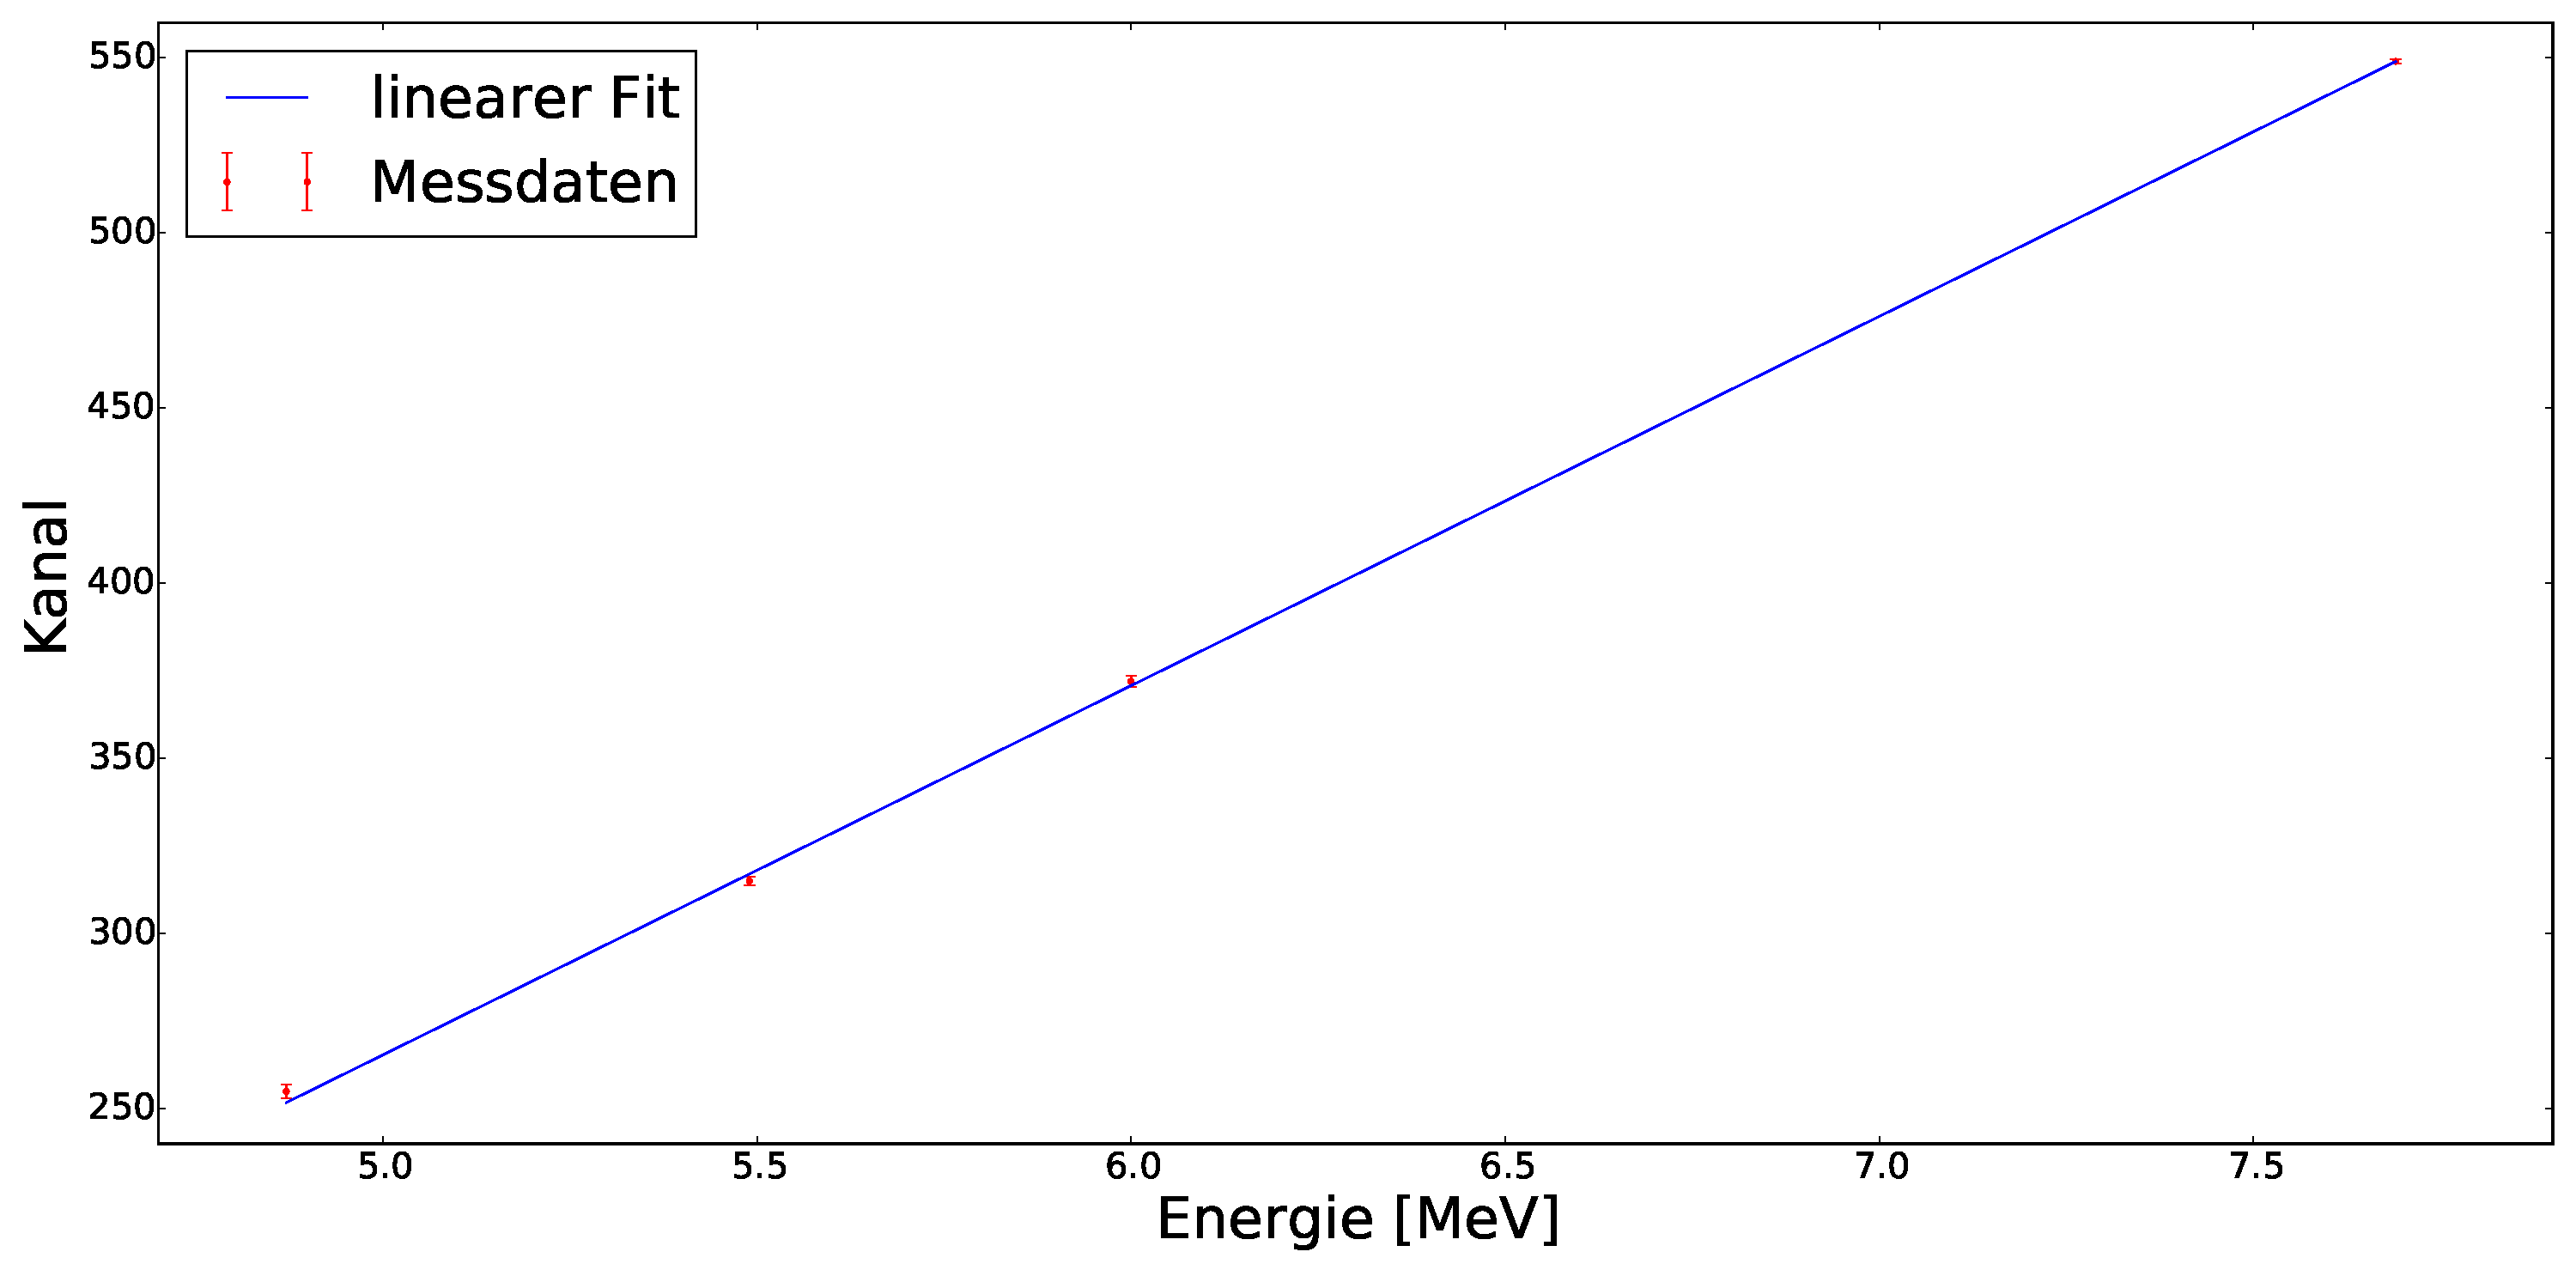
\includegraphics[scale=0.33]{linear_fit.pdf}
	\caption{Die bestimmten Kan�le gegen Zerfallsenergien mit linearem Fit}
	\label{fig:linear_fit}
\end{figure}


\begin{table}[H]
\centering
\caption{Parameter des Linearen-Fits}
\label{tab:linear-fit}
\begin{tabular}{|c|c|c|}
\hline Parameter & Wert & Fehler \\ 
\hline A [MeV] & 0,00949 & 0,00007 \\ 
\hline B [MeV]& 2,48 & 0,03 \\ 
\hline 
\end{tabular} 
\end{table}

\begin{align}
\label{eqn:energie-kanal}
E(k) = (0,00949 \pm 0,00007) \cdot k + (2,48 \pm 0,03)
\end{align}


\subsection{Druckmessung}
Die Kammer wird langsam bel�ftet und Spektren im Bereich von 100 Torr bis 800 Torr in 25 Torr Schritten aufgenommen, wobei der Druck w�hrend der Messung konstant gehalten wird. Ein Bar entspricht 750 Torr. Nach Gleichung \ref{eqn:reich_normal} kann die Strecke mit erh�htem Druck in die Strecke unter Normaldruck umgerechnet werden. Aus den Countrates in Abh�ngigkeit des Drucks kann der absolute Energieverlust und der Energieverlust pro Wegst�ck bei Normaldruck bestimmt werden. F�r den Energieverlust pro Wegst�ck wird ein Verhalten nach Gleichung \ref{eqn:reich_normal} erwartet. Die Peaks der Spektren werden wie zuvor mit einem Mulit-Gauss gefittet. Eine Messung wurde �ber einen Zeitraum von 180s durchgef�hrt.

\subsection{Energieverlust}
Der Energieverlust pro Strecke wird nach Gleichung \ref{eqn:verlust} berechnet.

\begin{align}
\label{eqn:verlust}
\frac{dE}{dx} = \frac{E_1 - E_2}{x_1 - x_2}
\end{align}

Dabei ergibt sich der Fehler nach Gleichung \ref{eqn:delta_verlust}.

\begin{align}
\label{eqn:delta_verlust}
\Delta \frac{dE}{dx} = \sqrt{\left( \frac{\Delta dE}{dx} \right)^2 + \left( \frac{\Delta dx \cdot dE}{dx^2} \right)^2 }
\end{align}

Die Wegdifferenz wurde mit Gleichung \ref{eqn:reich_normal} bestimmt, dabei ist P$_{normal}$ = 760 Torr und \mbox{x$_{normal}$ = 6 cm}. Die Energie wurde mit Gleichung \ref{eqn:energie-kanal} bestimmt. Die Energie wurde �ber den Mittelwert Gleichung \ref{eqn:e_mittel} bestimmt.  Der Fehler ist in Gleichung \ref{eqn:delta_e_mittel} angegeben.

\begin{align}
\label{eqn:e_mittel}
\bar{E} = \frac{E_1 + E_2}{2}
\end{align}

\begin{align}
\label{eqn:delta_e_mittel}
\Delta \bar{E} = \sqrt{ \left( \frac{\Delta E_1}{2} \right)^2 + \left( \frac{\Delta E_2}{2} \right)^2}
\end{align}

Die bestimmten Peakpositonen in Abh�ngigkeit vom Druck sind in Tabelle \ref{tab:multi-fit-erg} aufgetragen. Tr�gt man nun $\frac{dE}{dx}$ gegen $dE$ auf, erwartet man das von der Bethe-Bloch-Formel beschriebene Verhalten. Die Bethe-Bloch-Formel ist in Gleichung \ref{eqn:bethe-bloch} zu sehen. Da nur der Verlauf der Daten von intresse ist und nicht die Werte der einzelnen Parameter, k�nnen die Messdaten mit einem vereinfachten Modell, Gleichung \ref{eqn:bethe-bloch-einfach} gefittet werden. Dabei wird ein linearer Zusammenhang zwischen der Energie und dem Geschwindigkeitsquadrat der Teilchen angenommen ($E_{kin} \sim v^2$).

\begin{align}
\label{eqn:bethe-bloch-einfach}
\frac{dE}{dx} = \frac{A}{\beta^2} \left[ ln \left( B \cdot \beta^2 \right) - \beta^2 \right]
\end{align}

In Abb. \ref{fig:bethe_1} ist $\frac{dE}{dx}$ gegen $dE$ f�r den 4,871 MeV Peak aufgetragen, die Werte des Fits sind in Tabelle \ref{tab:bethe_fit_1} zu sehen. 

\begin{table}[H]
\centering
\caption{Fitwerte f�r den 4,871 MeV Peak nach Gleichung \ref{eqn:bethe-bloch-einfach}}
\label{tab:bethe_fit_1}
\begin{tabular}{|c|c|}
\hline Parameter & Wert \\ 
\hline A & 1,8 $\pm$ 0,2 \\ 
\hline B & 3,8 $\pm$ 0,5 \\ 
\hline $\chi_{red}^2$ & 8,4 \\ 
\hline 
\end{tabular} 
\end{table}

\begin{figure}[H]
	\centering
  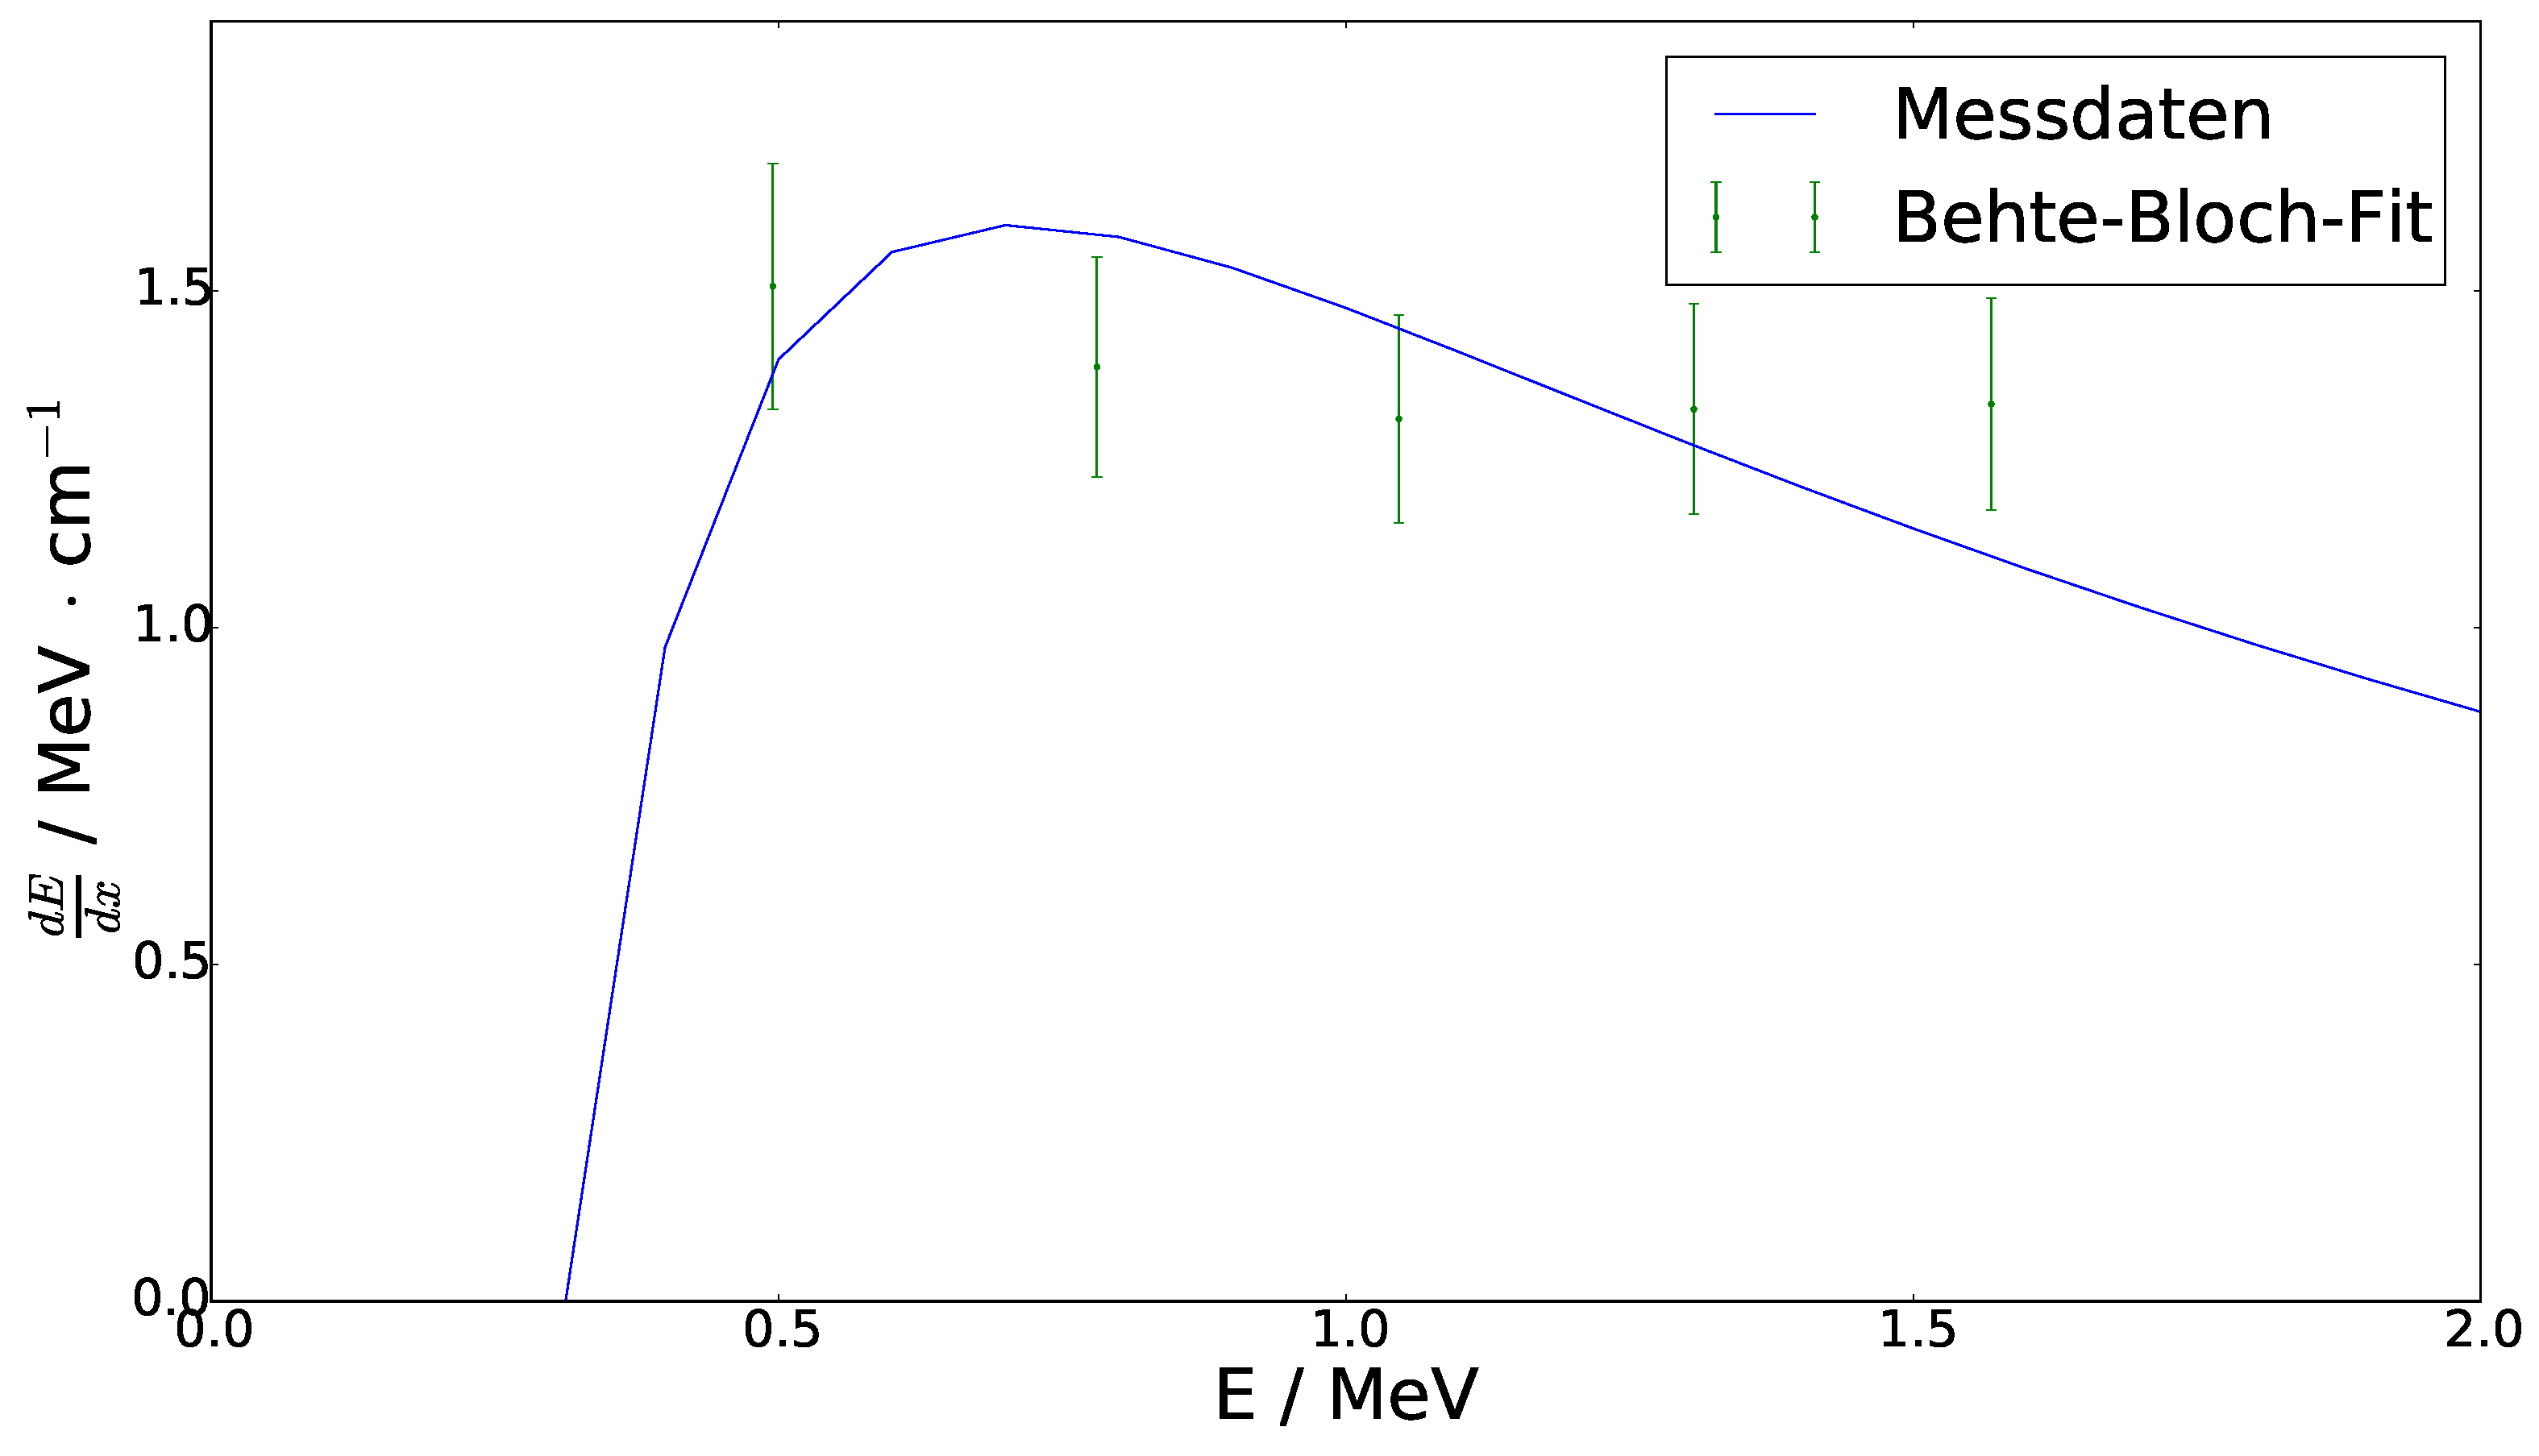
\includegraphics[scale=0.33]{bethebloch_1.pdf}
	\caption{Es ist $\frac{dE}{dx}$ gegen $dE$ aufgetragen, es wird ein Verlauf nach der Bethe-Bloch-Formel (Gleichung \ref{eqn:bethe-bloch}) erwartet. Aus dem Fit mit Gleichung \ref{eqn:bethe-bloch-einfach} ergibt sich ein reduziertes Chiquadrat $\chi_{red}^2$ von 8,4.}
	\label{fig:bethe_1}
\end{figure}


In Abb. \ref{fig:bethe_2} ist $\frac{dE}{dx}$ gegen $dE$ f�r den 5,49 MeV Peak aufgetragen, die Werte des Fits sind in Tabelle \ref{tab:bethe_fit_2} zu sehen. 

\begin{table}[H]
\centering
\caption{Fitwerte f�r den 5,49 MeV Peak nach Gleichung \ref{eqn:bethe-bloch-einfach}}
\label{tab:bethe_fit_2}
\begin{tabular}{|c|c|}
\hline Parameter & Wert \\ 
\hline A & 2,1 $\pm$ 0,1 \\ 
\hline B & 3,2 $\pm$ 0,2 \\ 
\hline $\chi_{red}^2$ & 13,4 \\ 
\hline 
\end{tabular} 
\end{table}

\begin{figure}[H]
	\centering
  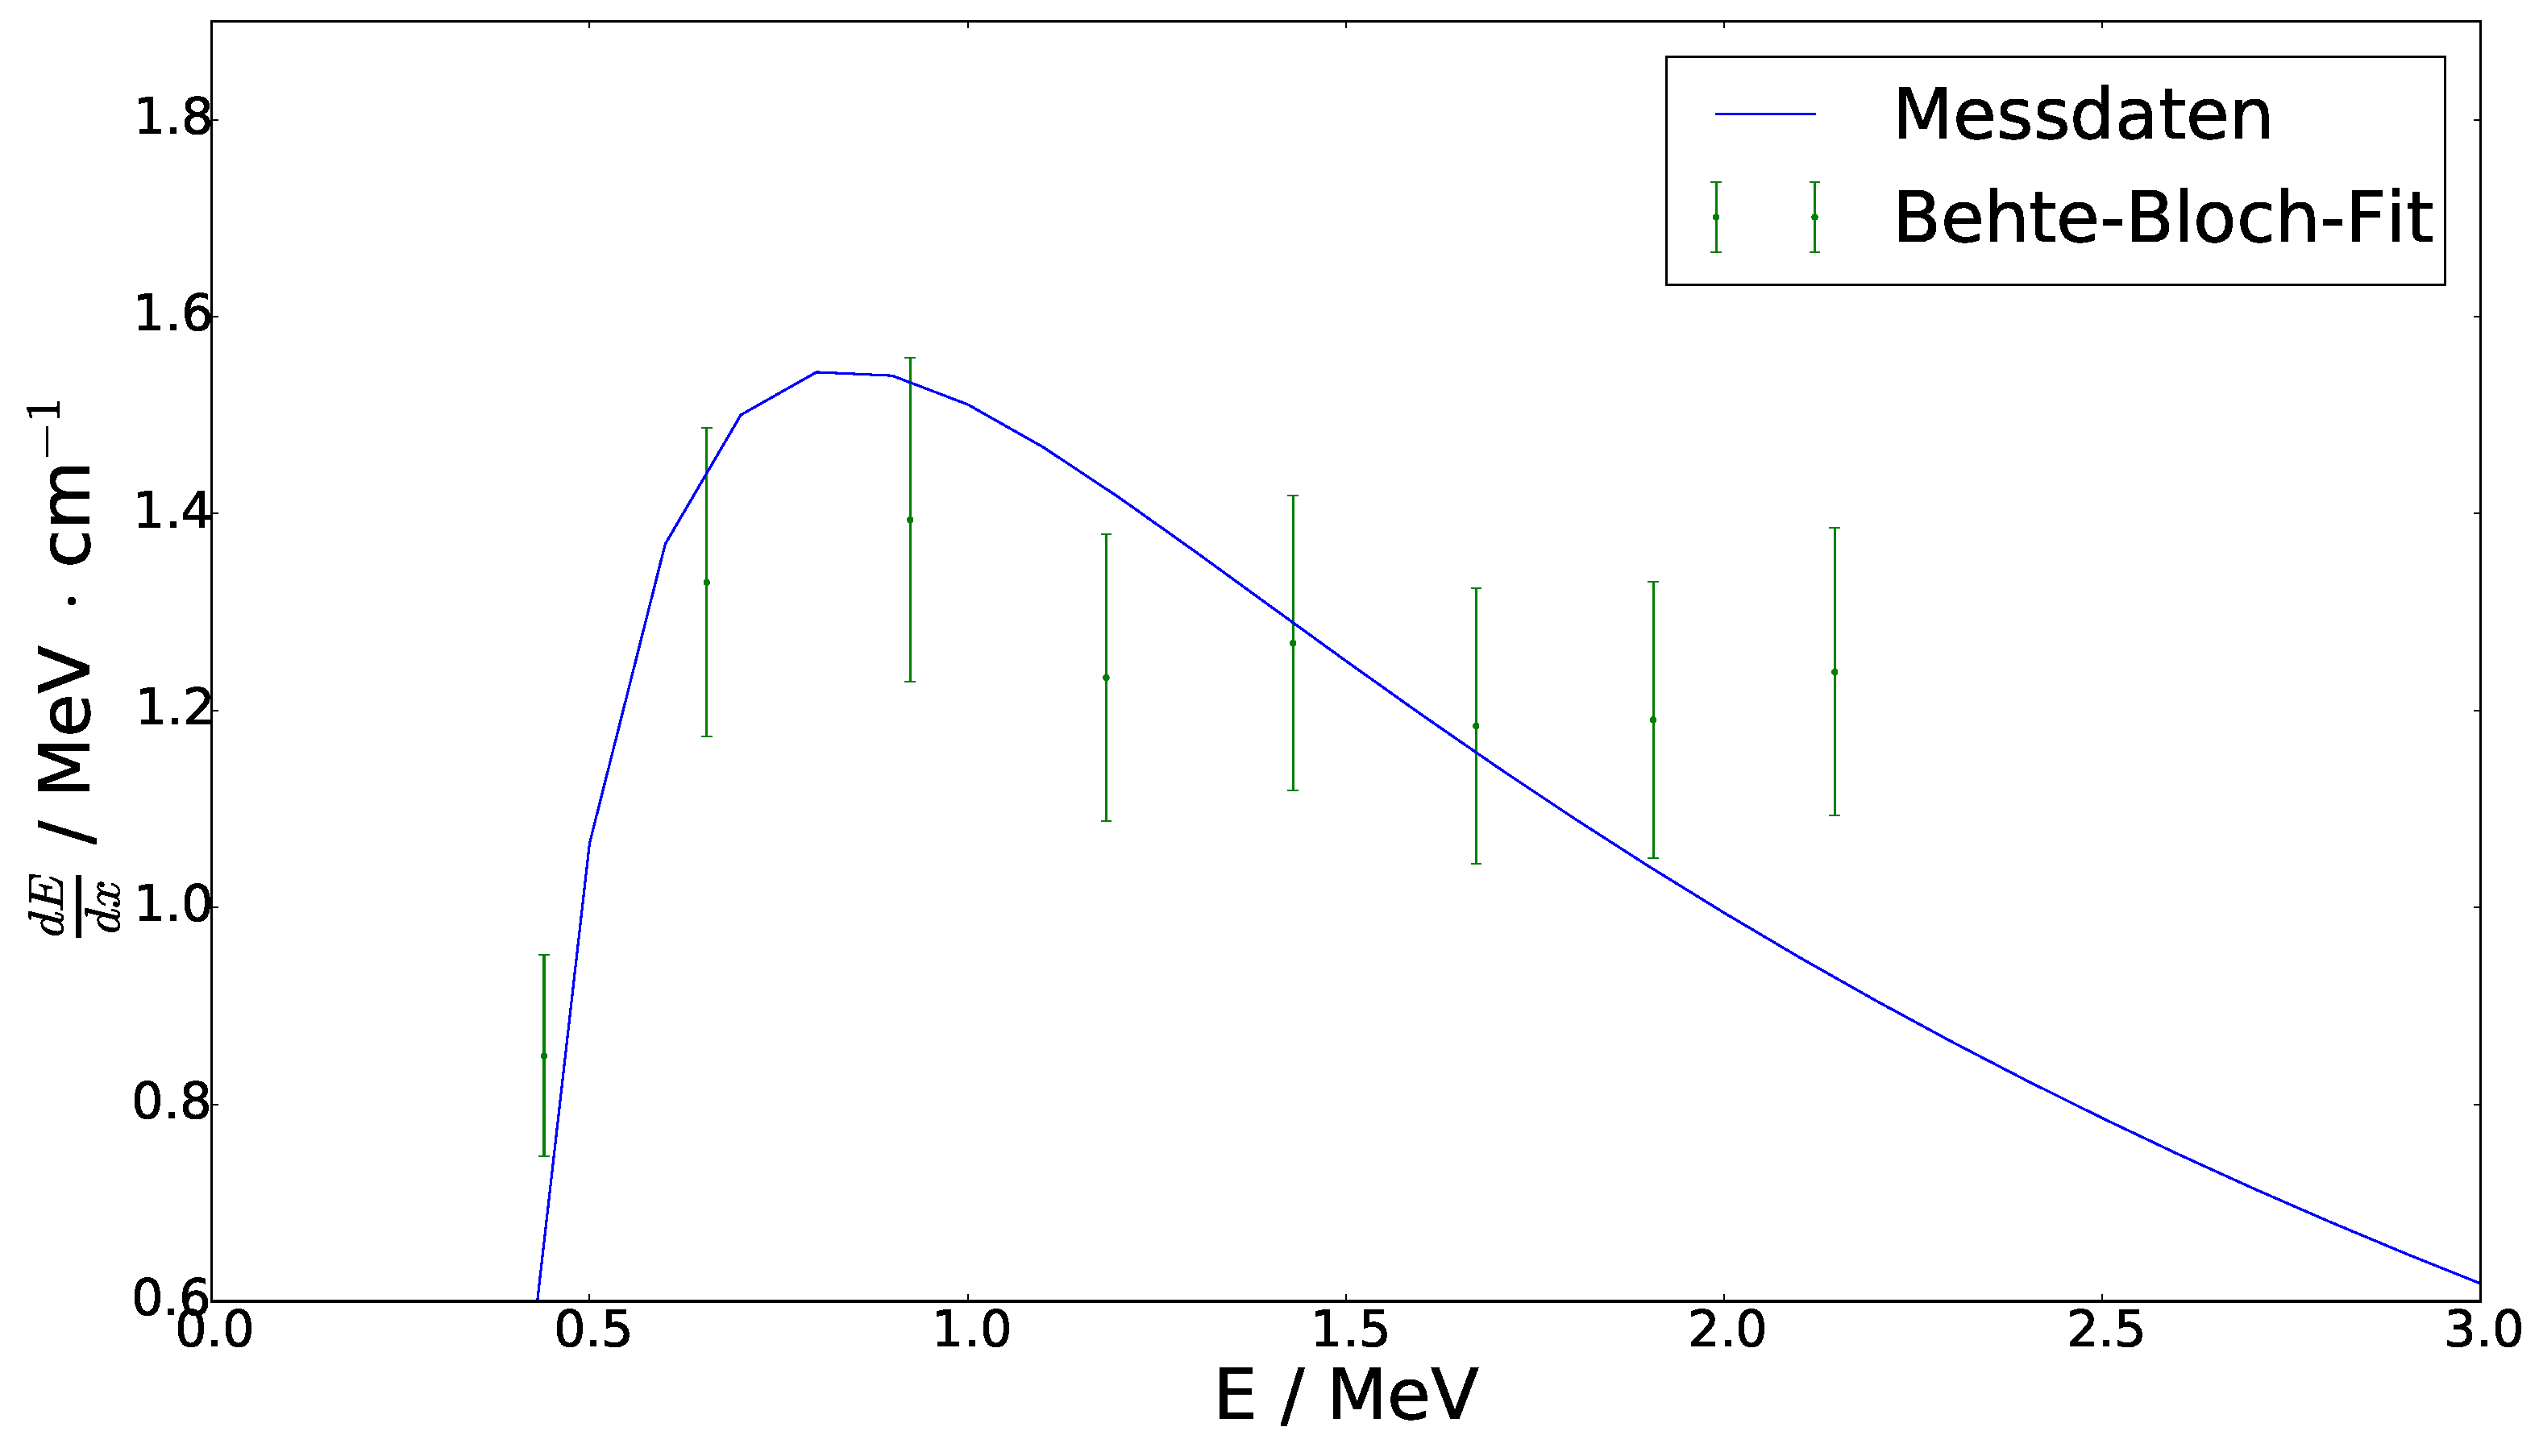
\includegraphics[scale=0.33]{bethebloch_2.pdf}
	\caption{Es ist $\frac{dE}{dx}$ gegen $dE$ f�r den 5,49 MeV Peak aufgetragen, es wird ein Verlauf nach der Bethe-Bloch-Formel (Gleichung \ref{eqn:bethe-bloch}) erwartet. Aus dem Fit mit Gleichung \ref{eqn:bethe-bloch-einfach} ergibt sich ein $\chi_{red}^2$ von 13,4.}
	\label{fig:bethe_2}
\end{figure}




In Abb. \ref{fig:bethe_3} ist $\frac{dE}{dx}$ gegen $dE$ f�r den 6 MeV Peak aufgetragen, die Werte des Fits sind in Tabelle \ref{tab:bethe_fit_3} zu sehen. 

\begin{table}[H]
\centering
\caption{Fitwerte f�r den 6 MeV Peak nach Gleichung \ref{eqn:bethe-bloch-einfach}}
\label{tab:bethe_fit_3}
\begin{tabular}{|c|c|}
\hline Parameter & Wert \\ 
\hline A & 2,0 $\pm$ 0,1 \\ 
\hline B & 3,5 $\pm$ 0,2 \\ 
\hline $\chi_{red}^2$ & 17,5 \\ 
\hline 
\end{tabular} 
\end{table}

\begin{figure}[H]
	\centering
  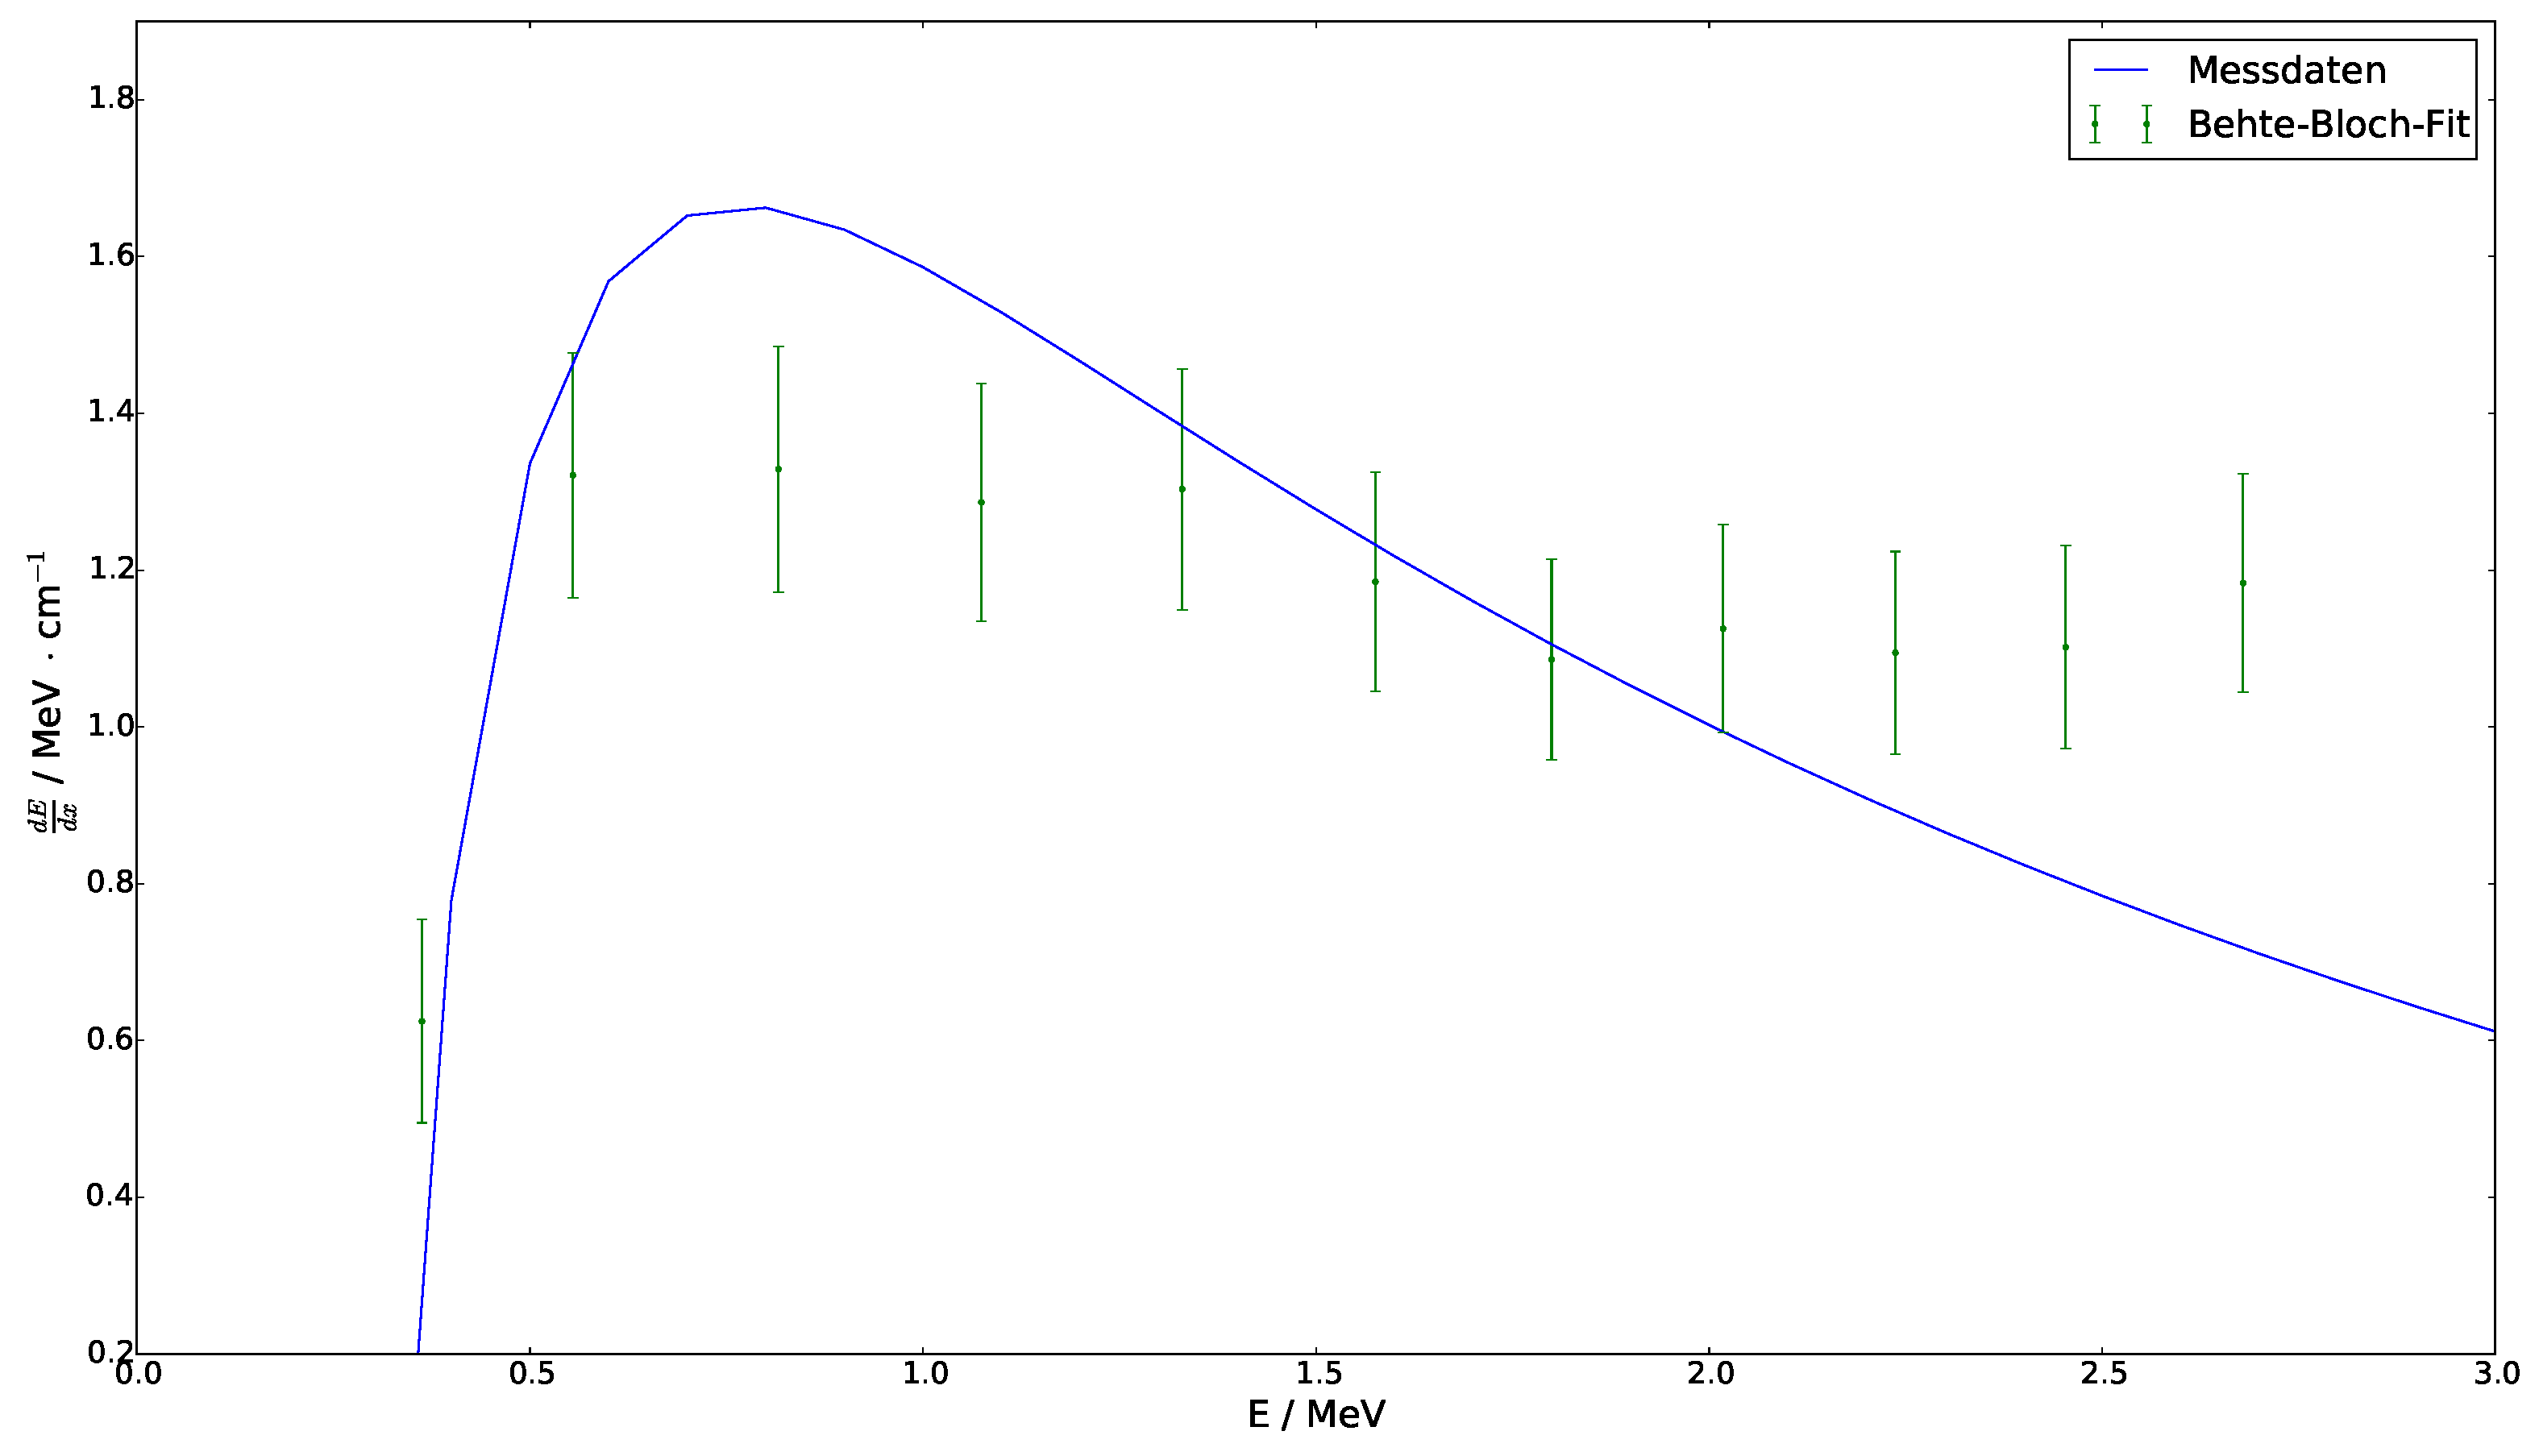
\includegraphics[scale=0.33]{bethebloch_3.pdf}
	\caption{Es ist $\frac{dE}{dx}$ gegen $dE$, f�r den 6 MeV Peak aufgetragen, es wird ein Verlauf nach der Bethe-Bloch-Formel (Gleichung \ref{eqn:bethe-bloch}) erwartet. Aus dem Fit mit Gleichung \ref{eqn:bethe-bloch-einfach} ergibt sich ein $\chi_{red}^2$ von 17,5.}
	\label{fig:bethe_3}
\end{figure}



In Abb. \ref{fig:bethe_4} ist $\frac{dE}{dx}$ gegen $dE$ f�r den 7,69 MeV Peak aufgetragen. Die Werte des Fits sind in Tabelle \ref{tab:bethe_fit_4} zu sehen. 

\begin{table}[H]
\centering
\caption{Fitwerte f�r den 7,69 MeV Peak nach Gleichung \ref{eqn:bethe-bloch-einfach}}
\label{tab:bethe_fit_4}
\begin{tabular}{|c|c|}
\hline Parameter & Wert \\ 
\hline A & 2,3 $\pm$ 0,2 \\ 
\hline B & 3,2 $\pm$ 0,3 \\ 
\hline $\chi_{red}^2$ & 30,9 \\ 
\hline 
\end{tabular} 
\end{table}

\begin{figure}[H]
	\centering
  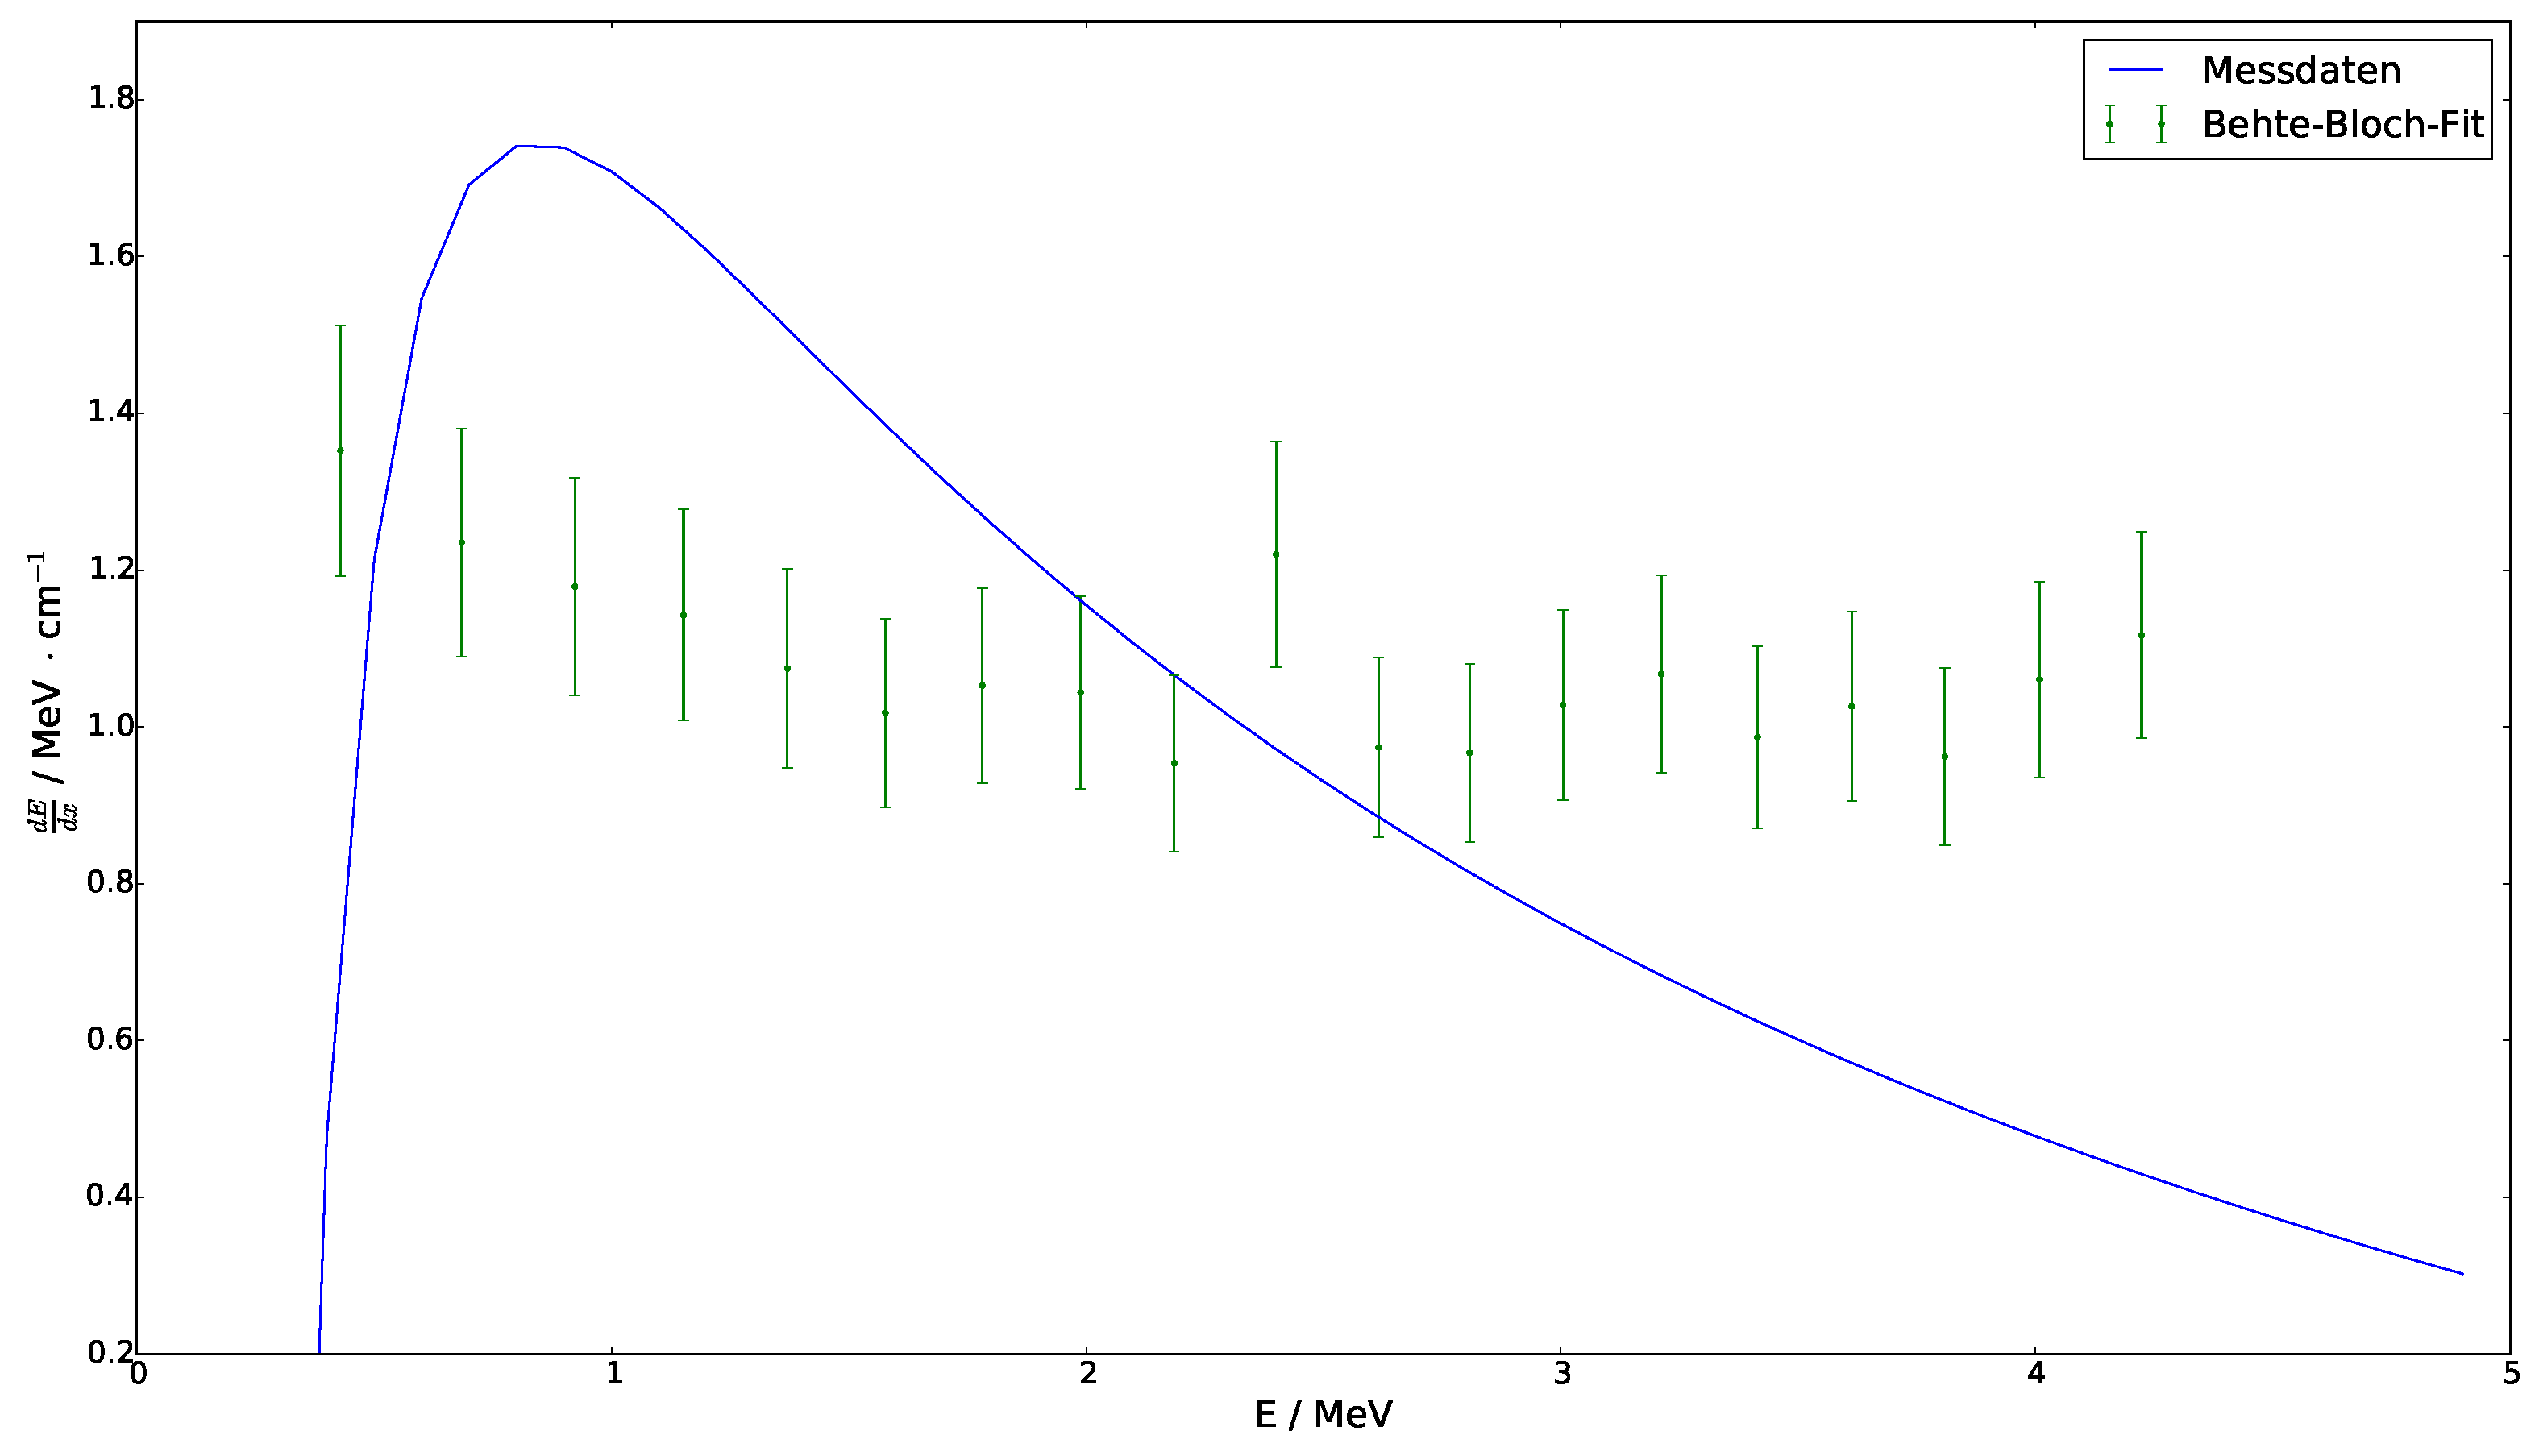
\includegraphics[scale=0.33]{bethebloch_4.pdf}
	\caption{Es ist $\frac{dE}{dx}$ gegen $dE$ f�r den 7,69 MeV Peak aufgetragen, es wird ein Verlauf nach der Bethe-Bloch-Formel (Gleichung \ref{eqn:bethe-bloch}) erwartet. Aus dem Fit mit Gleichung \ref{eqn:bethe-bloch-einfach} ergibt sich ein reduziertes Chiquadrat $\chi_{red}^2$ von 30,9.}
	\label{fig:bethe_4}
\end{figure}



Das $\chi_{red}^2$ liegt bei allen Fits weit oberhalb von 1, dabei f�llt auf, dass die ersten Werte besser an die Behte-Bloch-Kurve passen. Ab einem bestimmten Energiewert steigt $\frac{dE}{dx}$ bei allen Peaks. Der Energiewert, ab dem $\frac{dE}{dx}$ steigt, ist bei jedem Peak anders, weshalb ein systematischer Fehler ab einer bestimmten Messung ausgeschlossen werden kann. Die Quelle des Fehlers ist Unbekannt. Wie sich in Abschnitt \ref{subsec:bragg} zeigt, ist der Verlauf der Bragg-Kurven bei allen Messungen wie erwartet.

\subsection{Bragg-Kurve}
\label{subsec:bragg}
Tr�gt man $\frac{dE}{dx}$ gegen die zur�ckgelgete Strecke auf, so erwartet man ein Verhalten wie in Abb. \ref{fig:braggkurve}.

In Abb. \ref{fig:bragg_1} ist f�r den 4,87 MeV Peak $\frac{dE}{dx}$ gegen $x$ zusehen.

\begin{figure}[H]
	\centering
  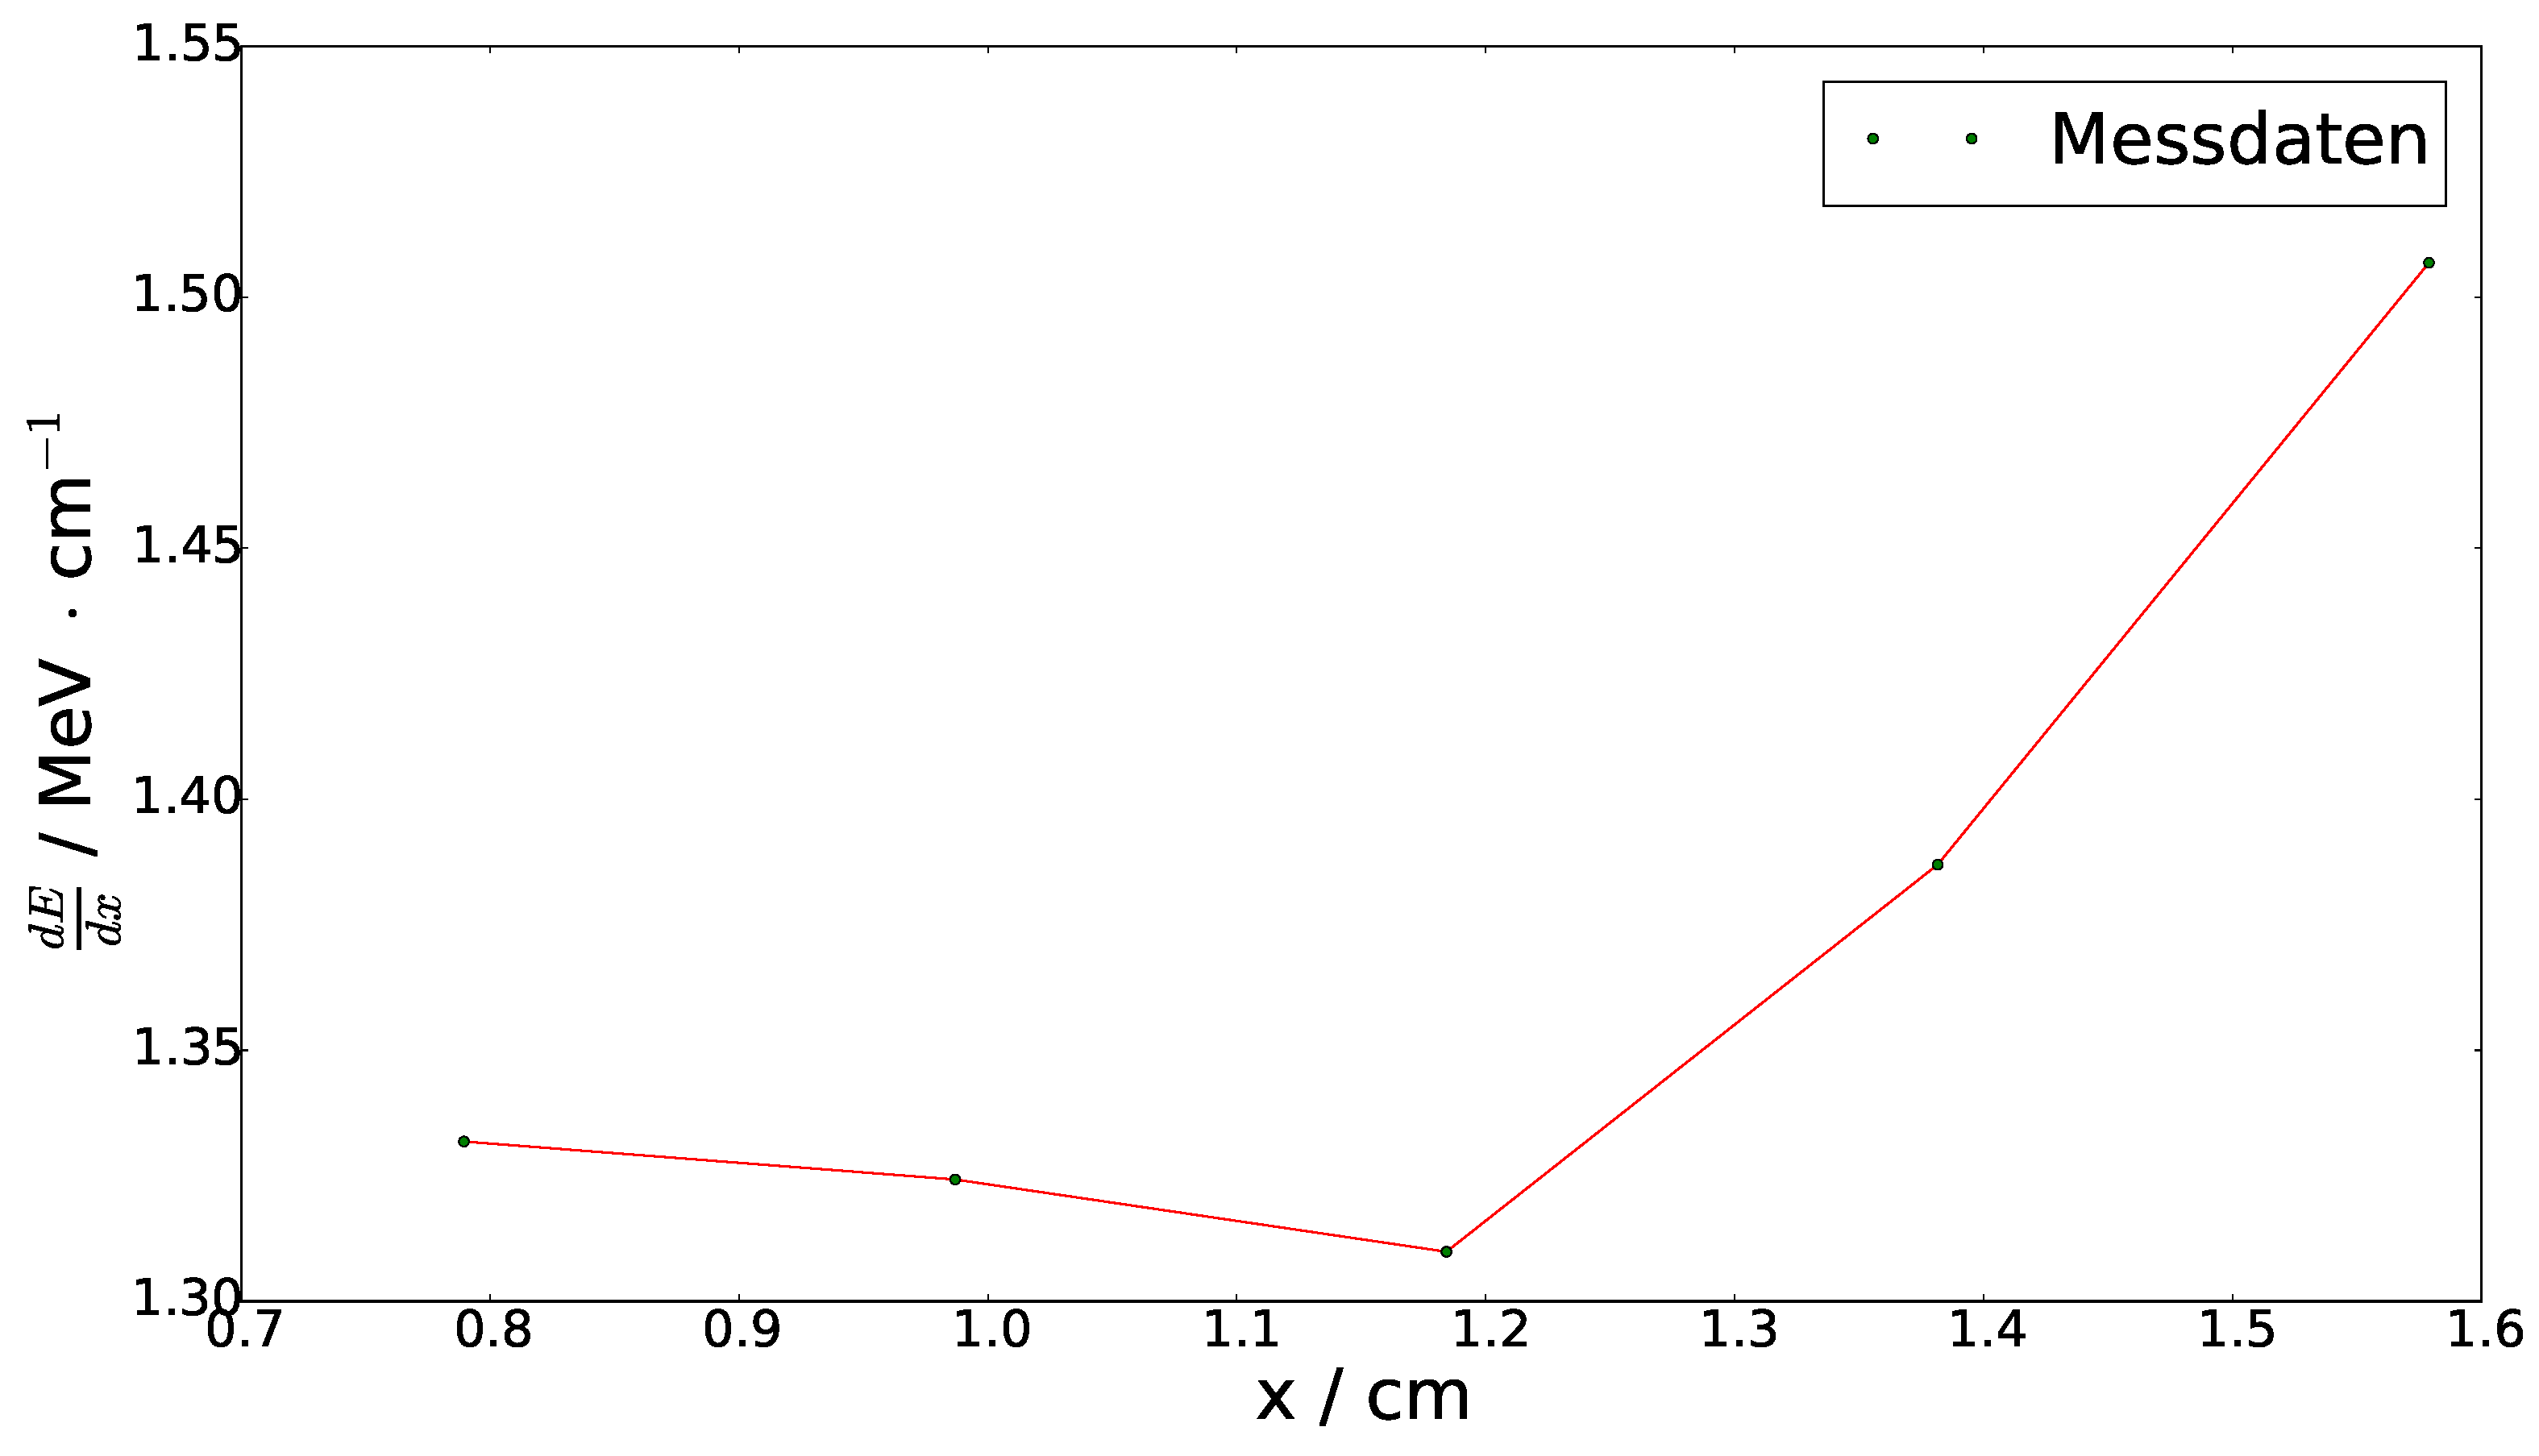
\includegraphics[scale=0.33]{bragg_kurve_1.pdf}
	\caption{Es wurde $\frac{dE}{dx}$ gegen $x$ aufgetragen. Der Anfang des Braggpeaks ist deutlich zu sehen}
	\label{fig:bragg_1}
\end{figure}

\noindent
In Abb. \ref{fig:bragg_2} ist f�r den 5,49 MeV Peak $\frac{dE}{dx}$ gegen $x$ aufgetragen.

\begin{figure}[H]
	\centering
  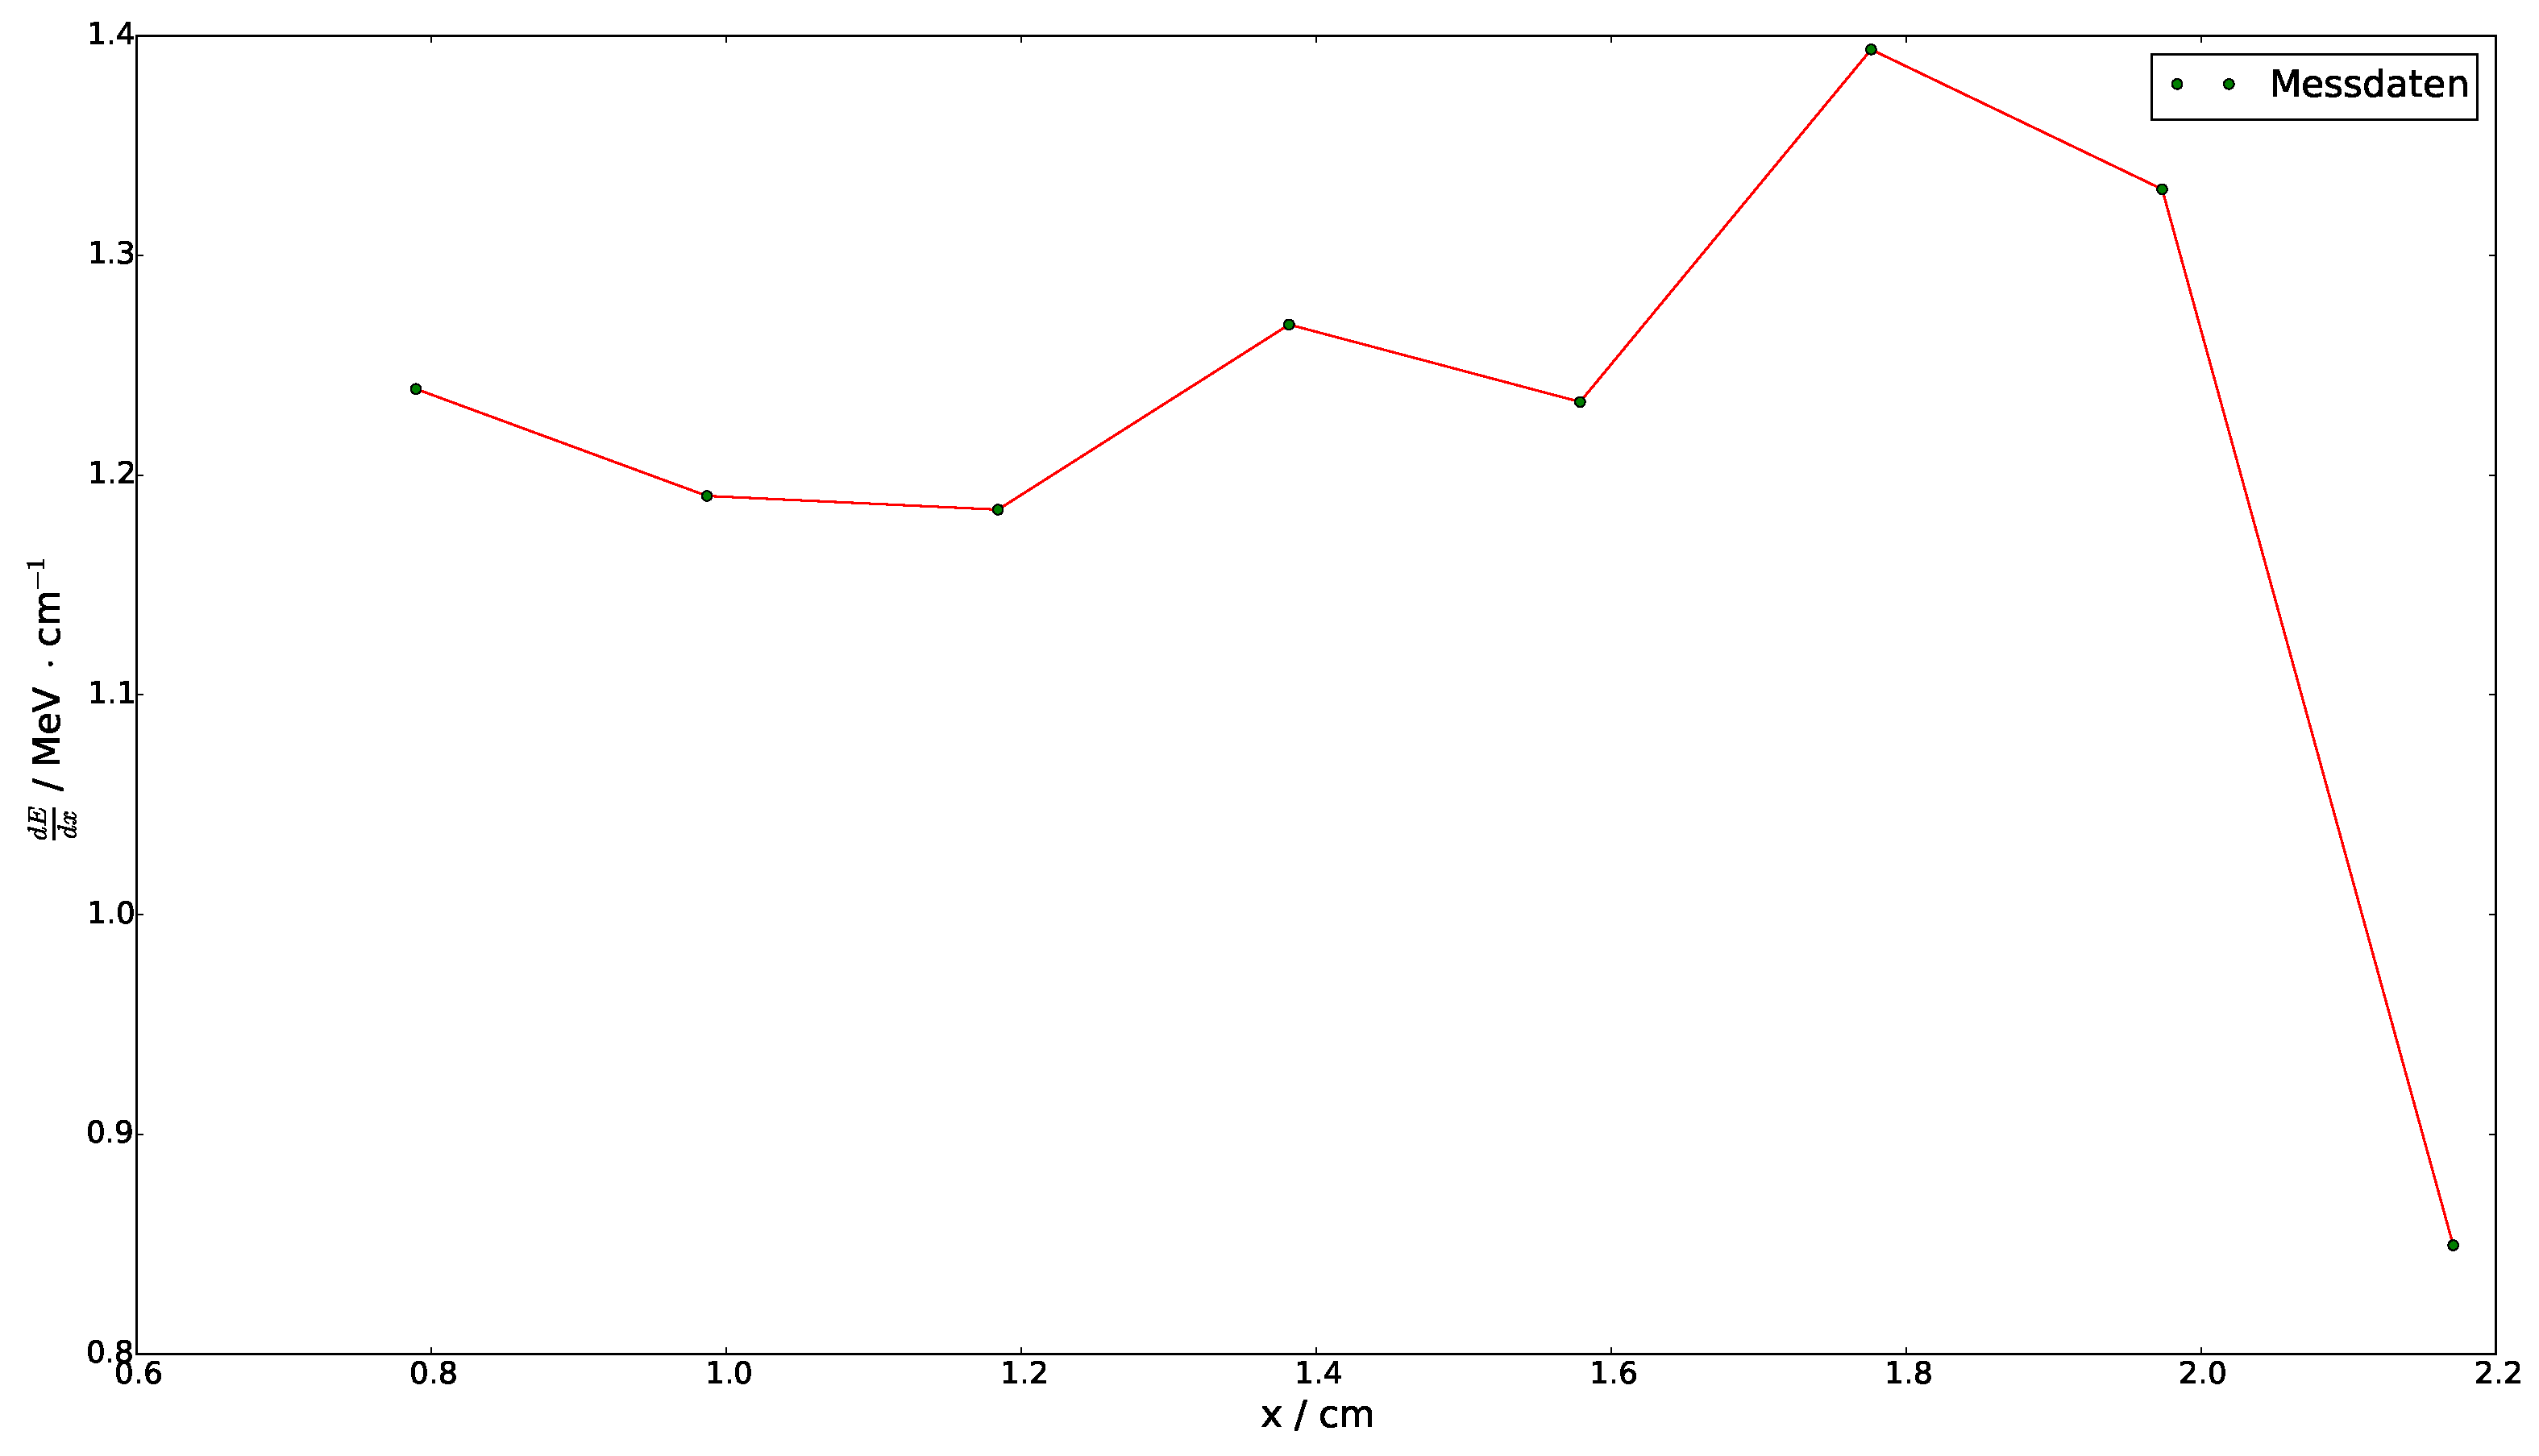
\includegraphics[scale=0.33]{bragg_kurve_2.pdf}
	\caption{$\frac{dE}{dx}$ gegen $x$ Aufgetragen. Der Braggpeak ist deutlich zu sehen}
	\label{fig:bragg_2}
\end{figure}

\noindent
In Abb. \ref{fig:bragg_3} ist f�r den 6 MeV Peak $\frac{dE}{dx}$ gegen $x$ aufgetragen.

\begin{figure}[H]
	\centering
  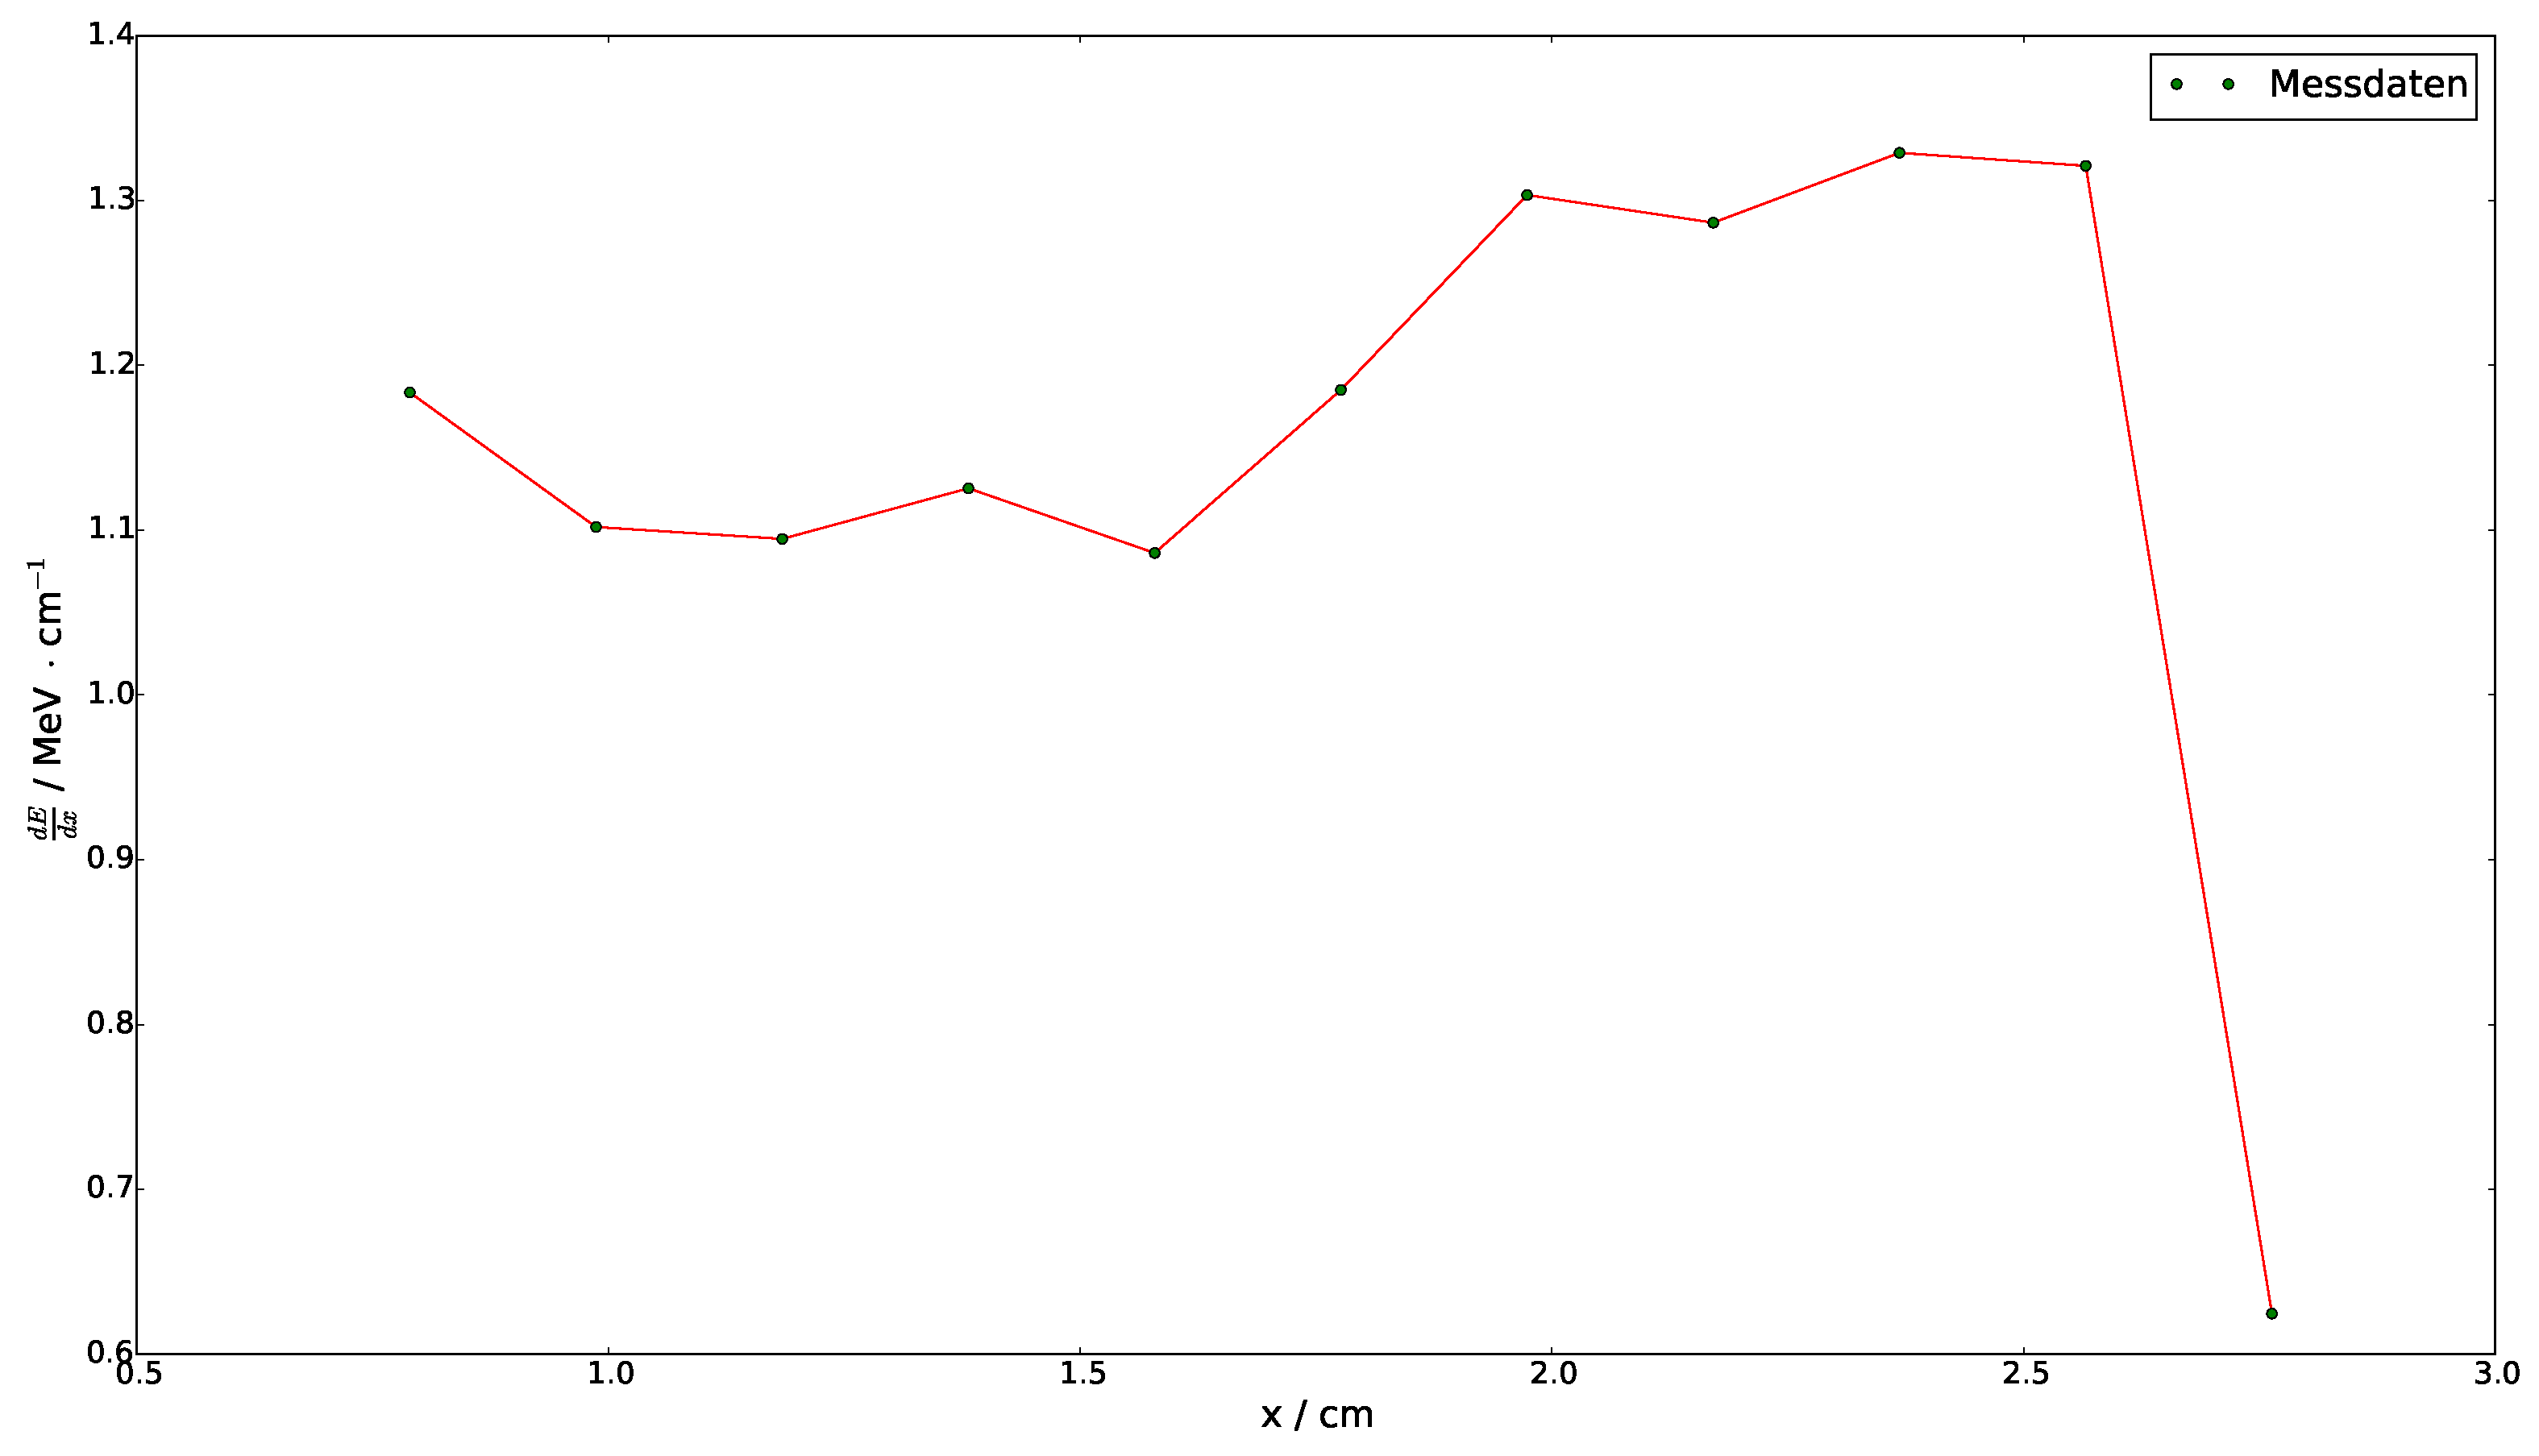
\includegraphics[scale=0.33]{bragg_kurve_3.pdf}
	\caption{Es wurde $\frac{dE}{dx}$ gegen $x$ aufgetragen. Der Braggpeak ist gut zu sehen}
	\label{fig:bragg_3}
\end{figure}


\noindent
In Abb. \ref{fig:bragg_4} ist f�r den 7,69 MeV Peak $\frac{dE}{dx}$ gegen $x$ zusehen.

\begin{figure}[H]
	\centering
  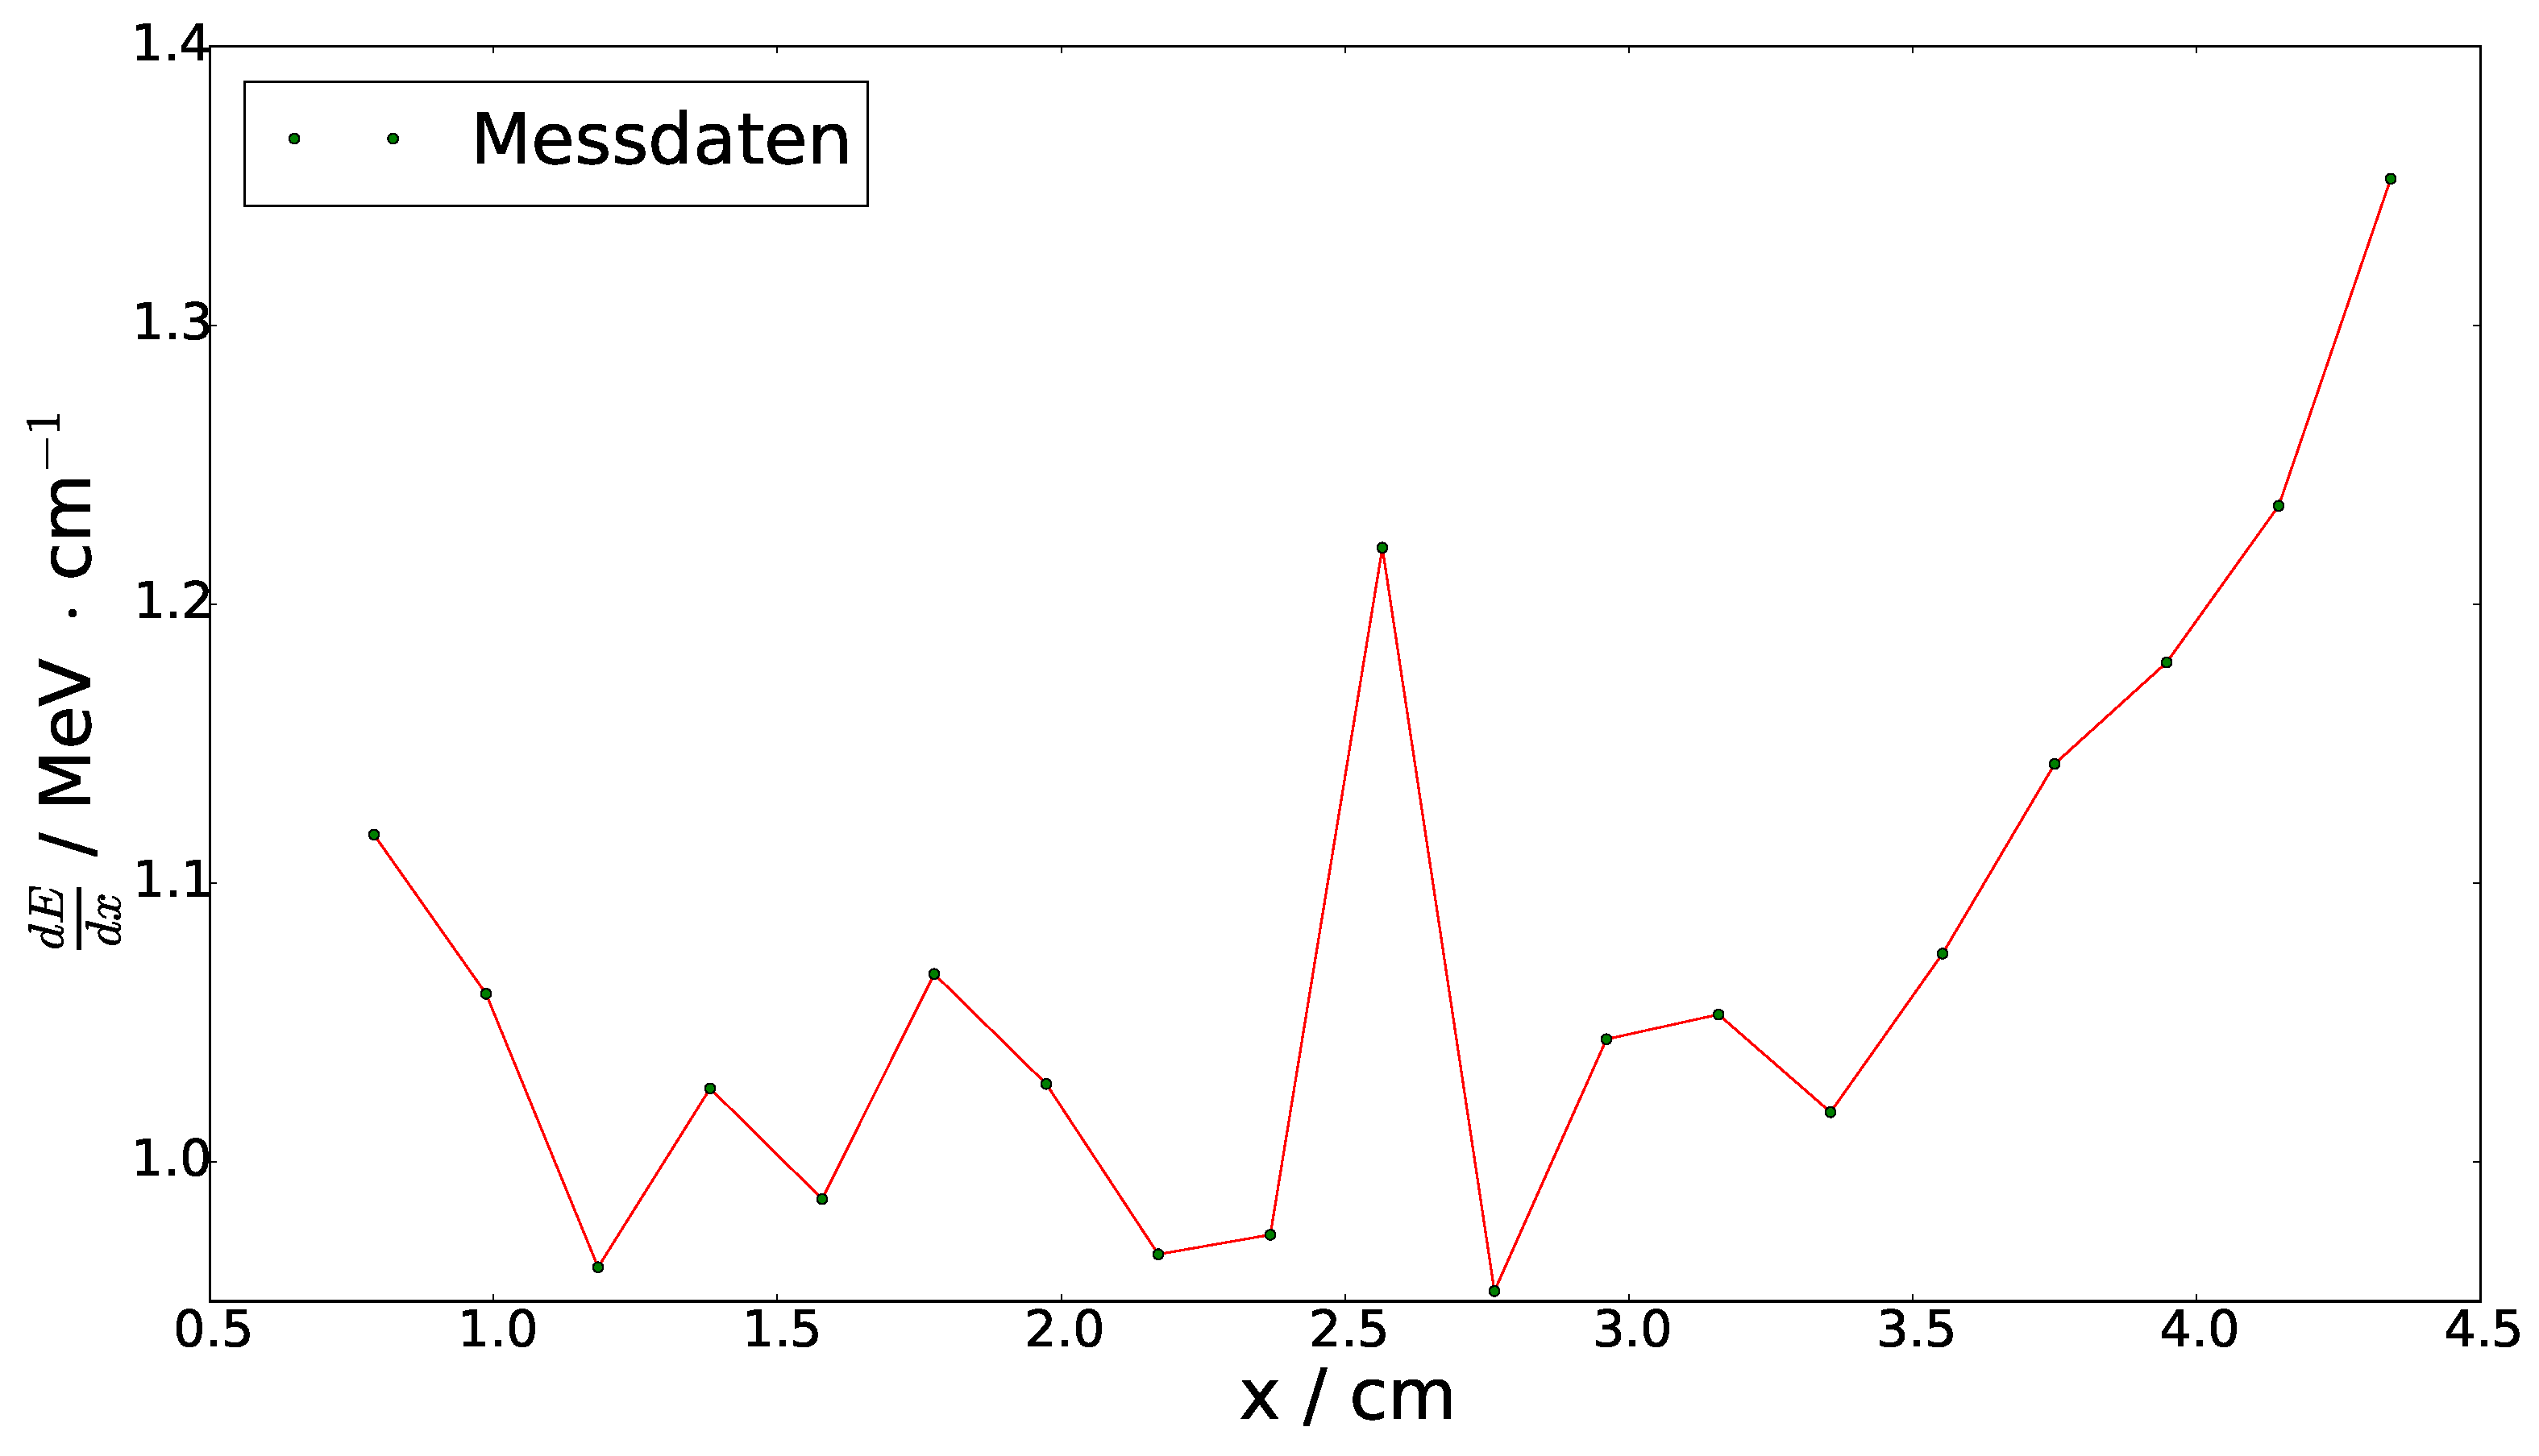
\includegraphics[scale=0.33]{bragg_kurve_4.pdf}
	\caption{$\frac{dE}{dx}$ wurde gegen $x$ aufgetragen. Der Anfang des Braggpeaks ist deutlich zu sehen, wobei die Herkunft des Ausrei�ers bei ca. 2,5 cm nicht klar ist.}
	\label{fig:bragg_4}
\end{figure}

Bei allen Plots ist die Form der Braggkurven zu erkennen. Vergleicht man Abb. \ref{fig:braggkurve} mit Abb. \ref{fig:bragg_2}, so f�llt auf, dass der erwartete Peak bei 3,7 cm liegt, der Peak in Abb. \ref{fig:bragg_2} jedoch bei ca. 1.8 cm liegt. Woher die Schiebung kommt ist nicht bekannt.
\section{Absorptionsverhalten von Aluminium und Papier}
%kurz das ziel dieses versuchsteiles ansprechen, damit keine zwei �berschriften direkt �bereinander stehen!
%bei schwierigeren versuchen kann auch der theoretische hintergrund erl�utert werden. (mit formeln, herleitungen und erkl�rungen)
In diesem Versuchsabschnitt soll das Absorptionsverhalten von Aluminium und Papier untersucht werden.

\subsection{Versuchsdurchf�hrung}
Es wird der selbe Aufbau wie in Abschnitt \ref{sec:energieverlust} verwendet. Zwischen Quelle und Detektor werden Papier bzw. Aluminium gelegt um die Absorption zu untersuchen. Zur Verf�gung stehen Papier mit 103$\mu$m und 32$\mu$m, sowie Aluminiumfolie mit einer Dicke von 13$\mu$m. Vor der Messung wird die Kammer auf 35 Torr evakuiert.

\subsection{Auswertung}

Die aufgenommenen Spektren sind in Abb. \ref{fig:ab_alu} (Aluminium), Abb. \ref{fig:ab_papier} (Papier) und Abb. \ref{fig:ab_biebel} (Biebelpapier) zu sehen. Die Alufolie schw�cht die $\alpha$-Strahlung ab, was an der Verschiebung nach links zu sehen ist. Das normale Papier Block die Strahlung nahezu vollst�ndig ab. Bei der Absorbtion durch das Biebelpapier, werde die ersten der Peaks zu einem verwaschen.


\begin{figure}[H]
	\centering
  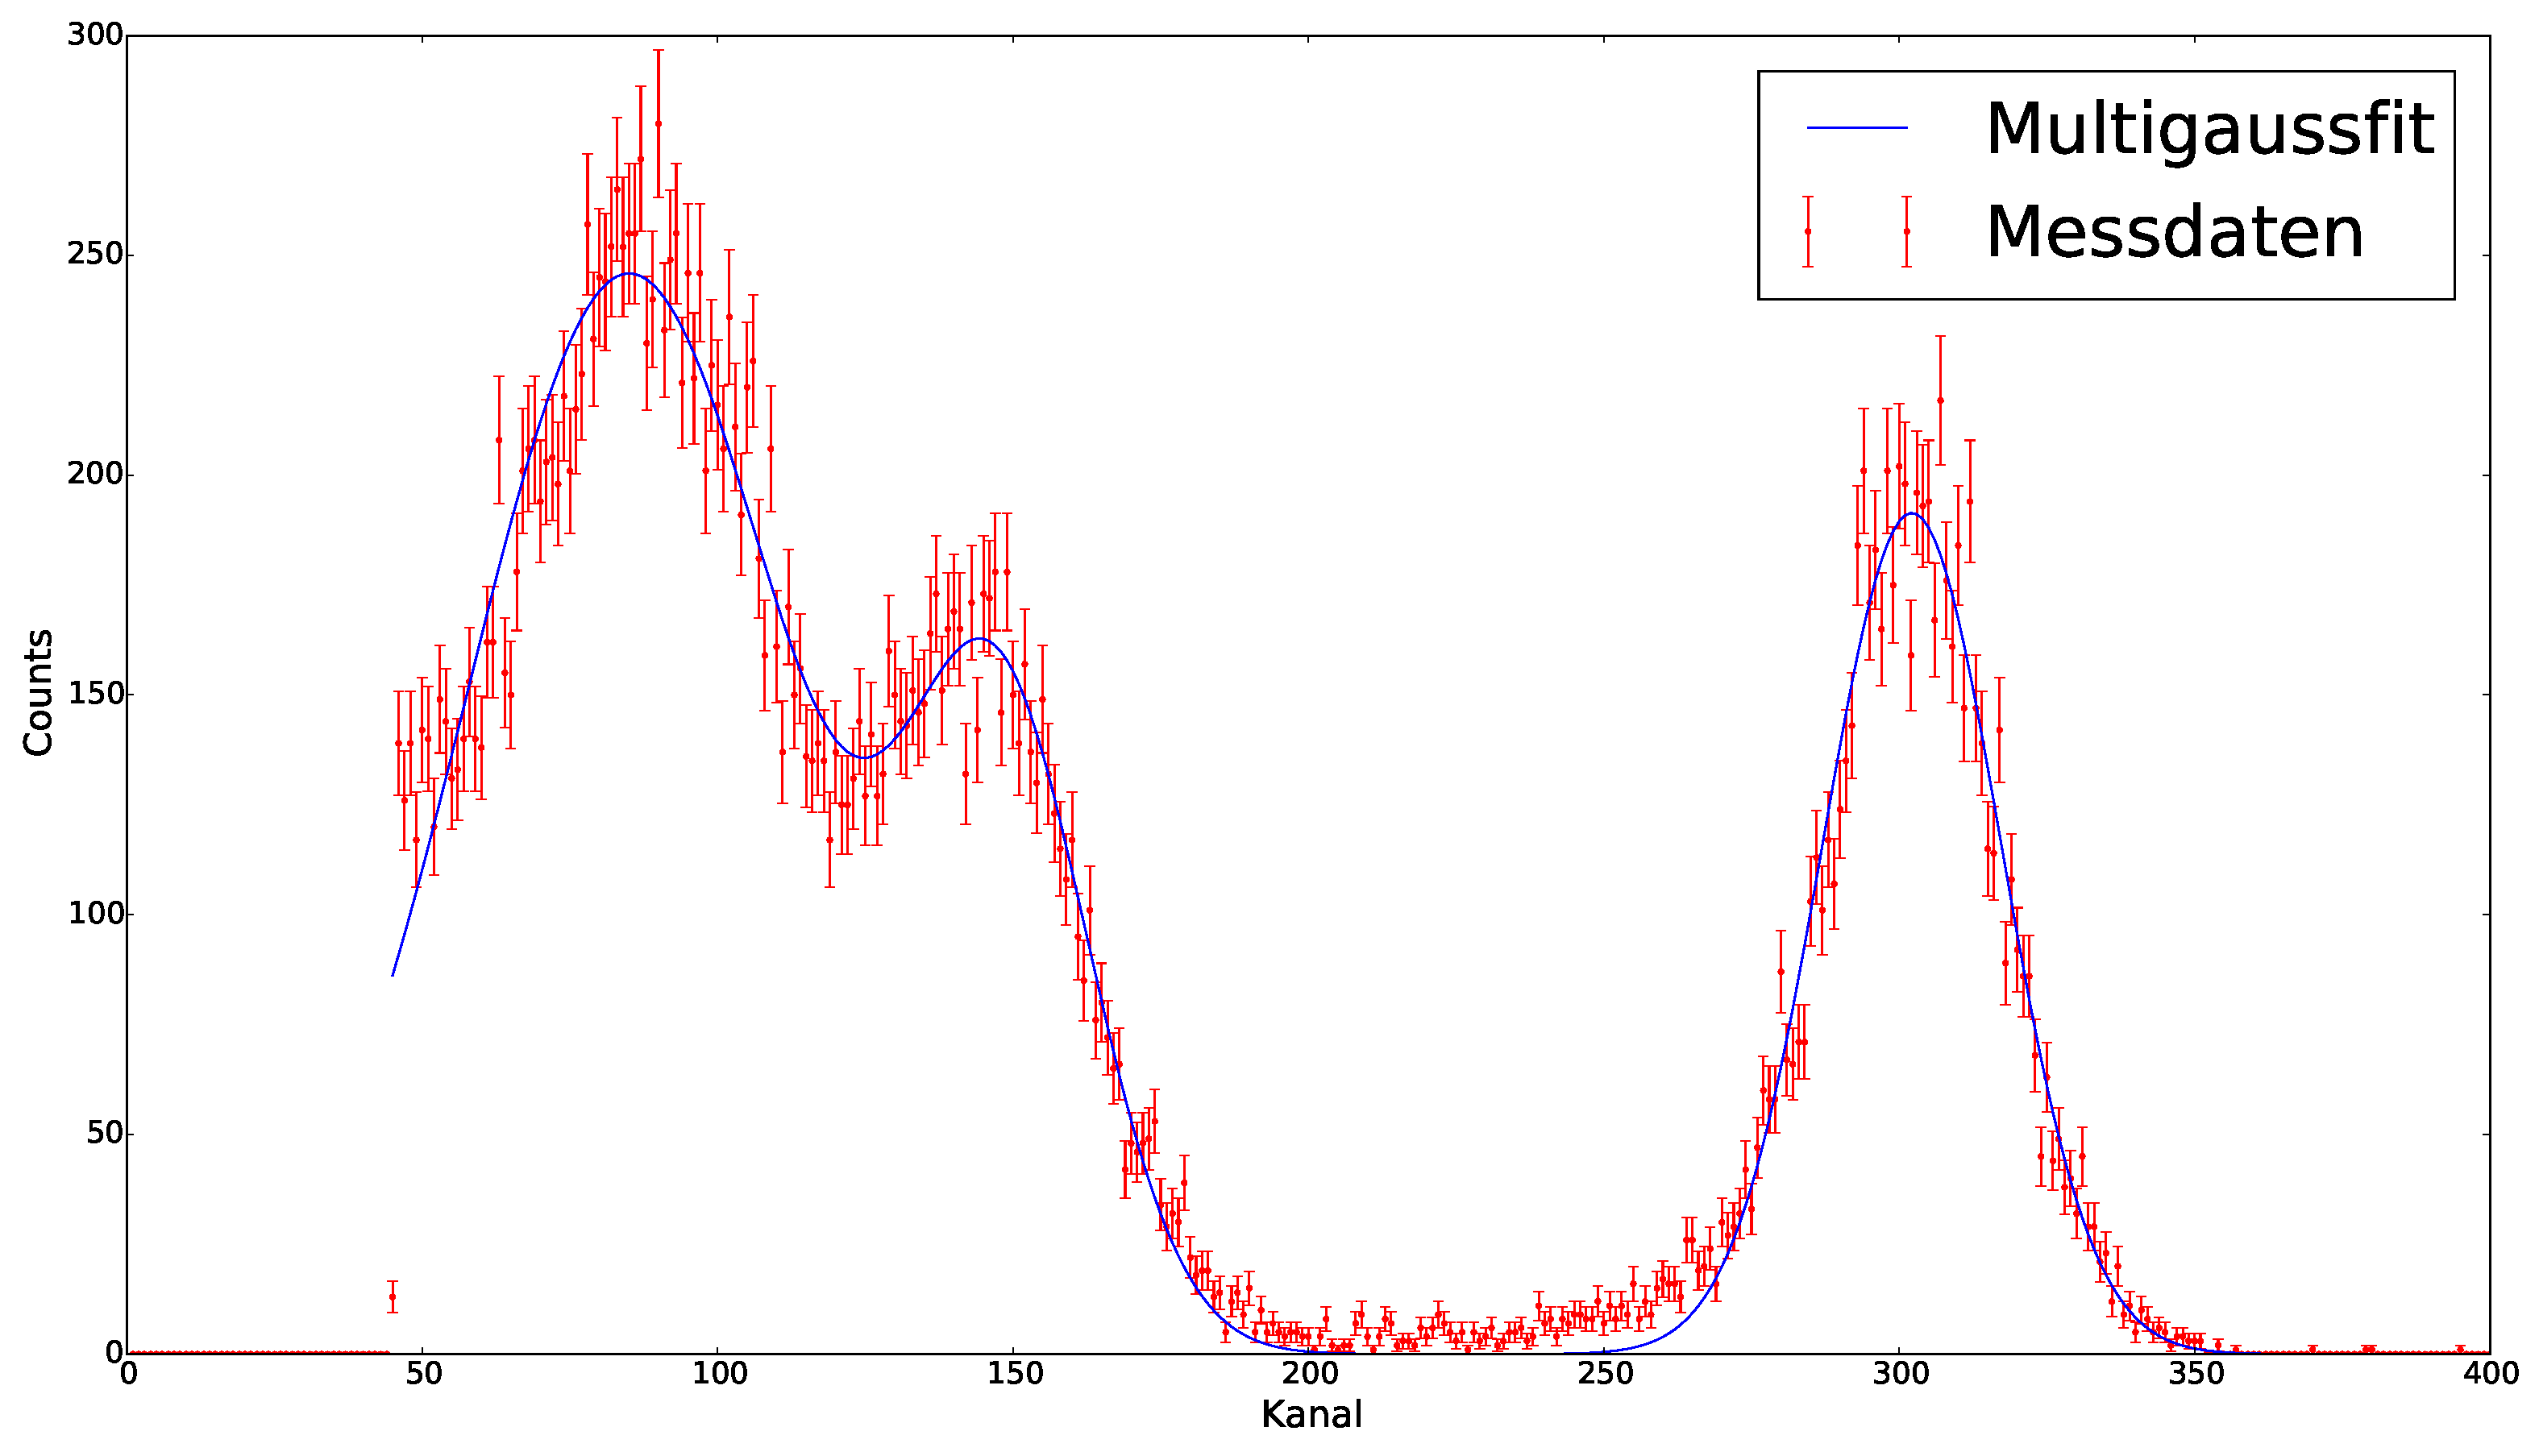
\includegraphics[scale=0.2]{ab_alu.pdf}
	\caption{Schematischer Aufbau des Streukammer}
	\label{fig:ab_alu}
\end{figure}

\begin{figure}[H]
	\centering
  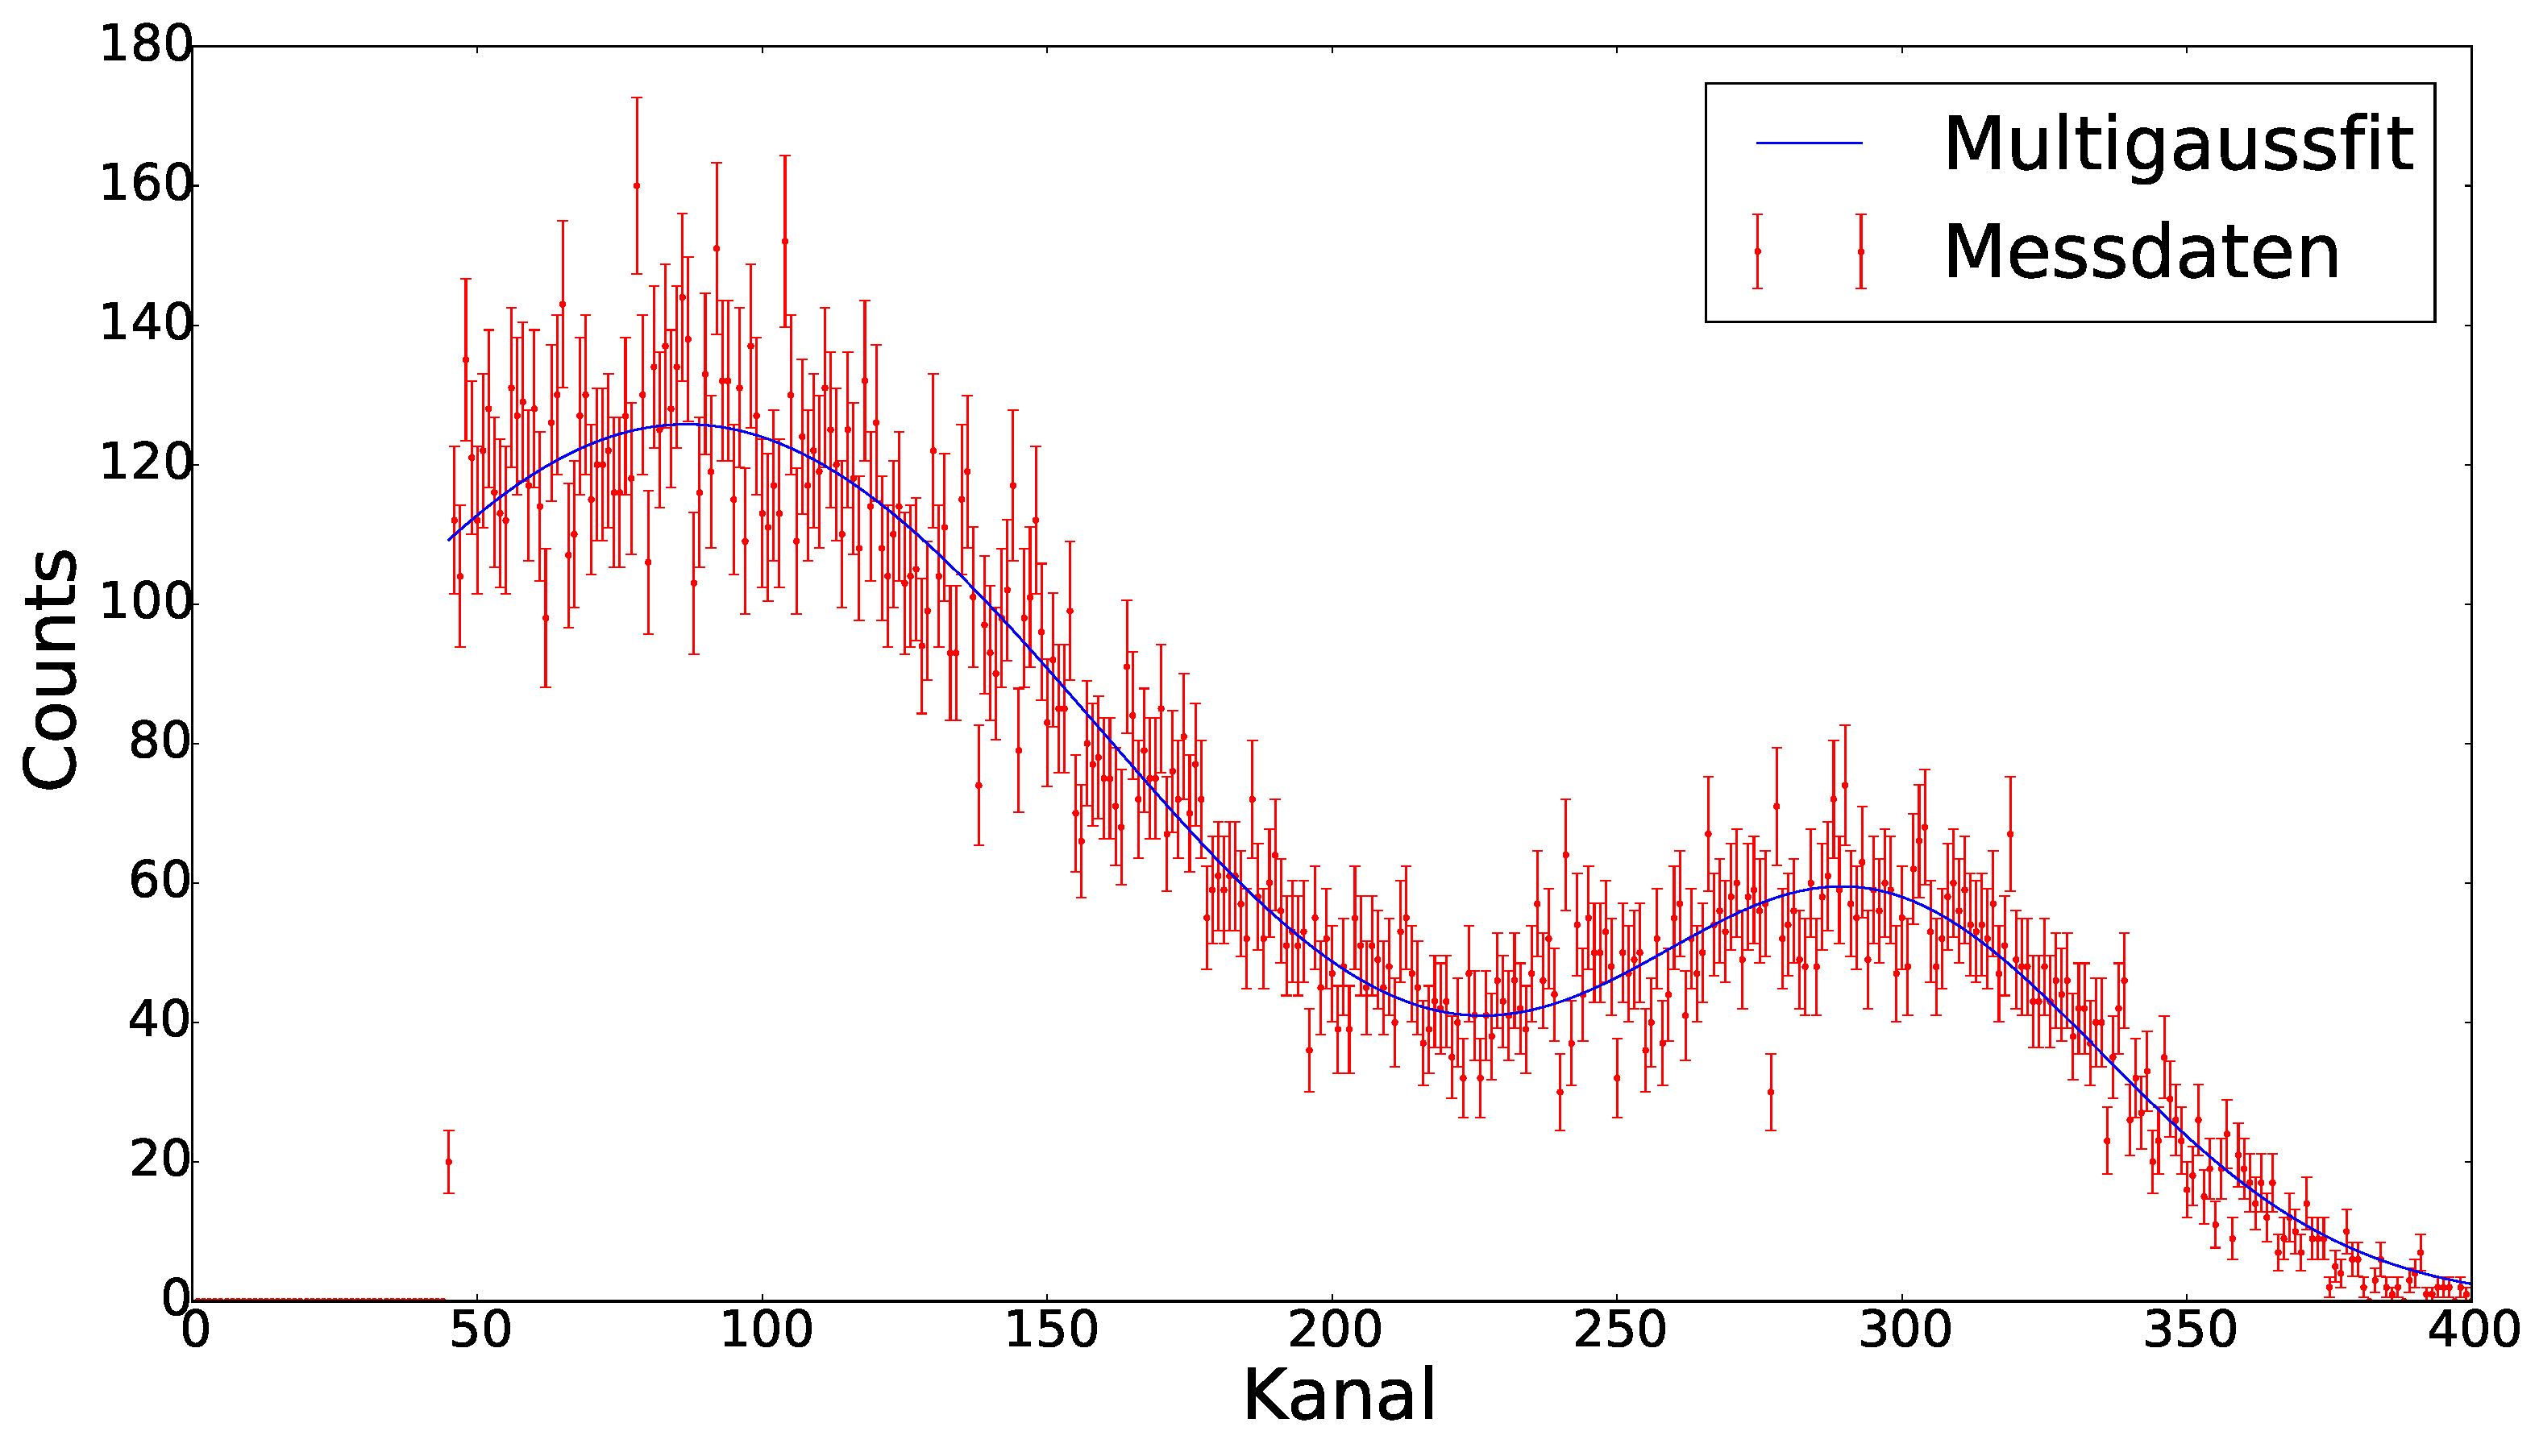
\includegraphics[scale=0.2]{ab_papier.pdf}
	\caption{Schematischer Aufbau des Streukammer}
	\label{fig:ab_papier}
\end{figure}

\begin{figure}[H]
	\centering
  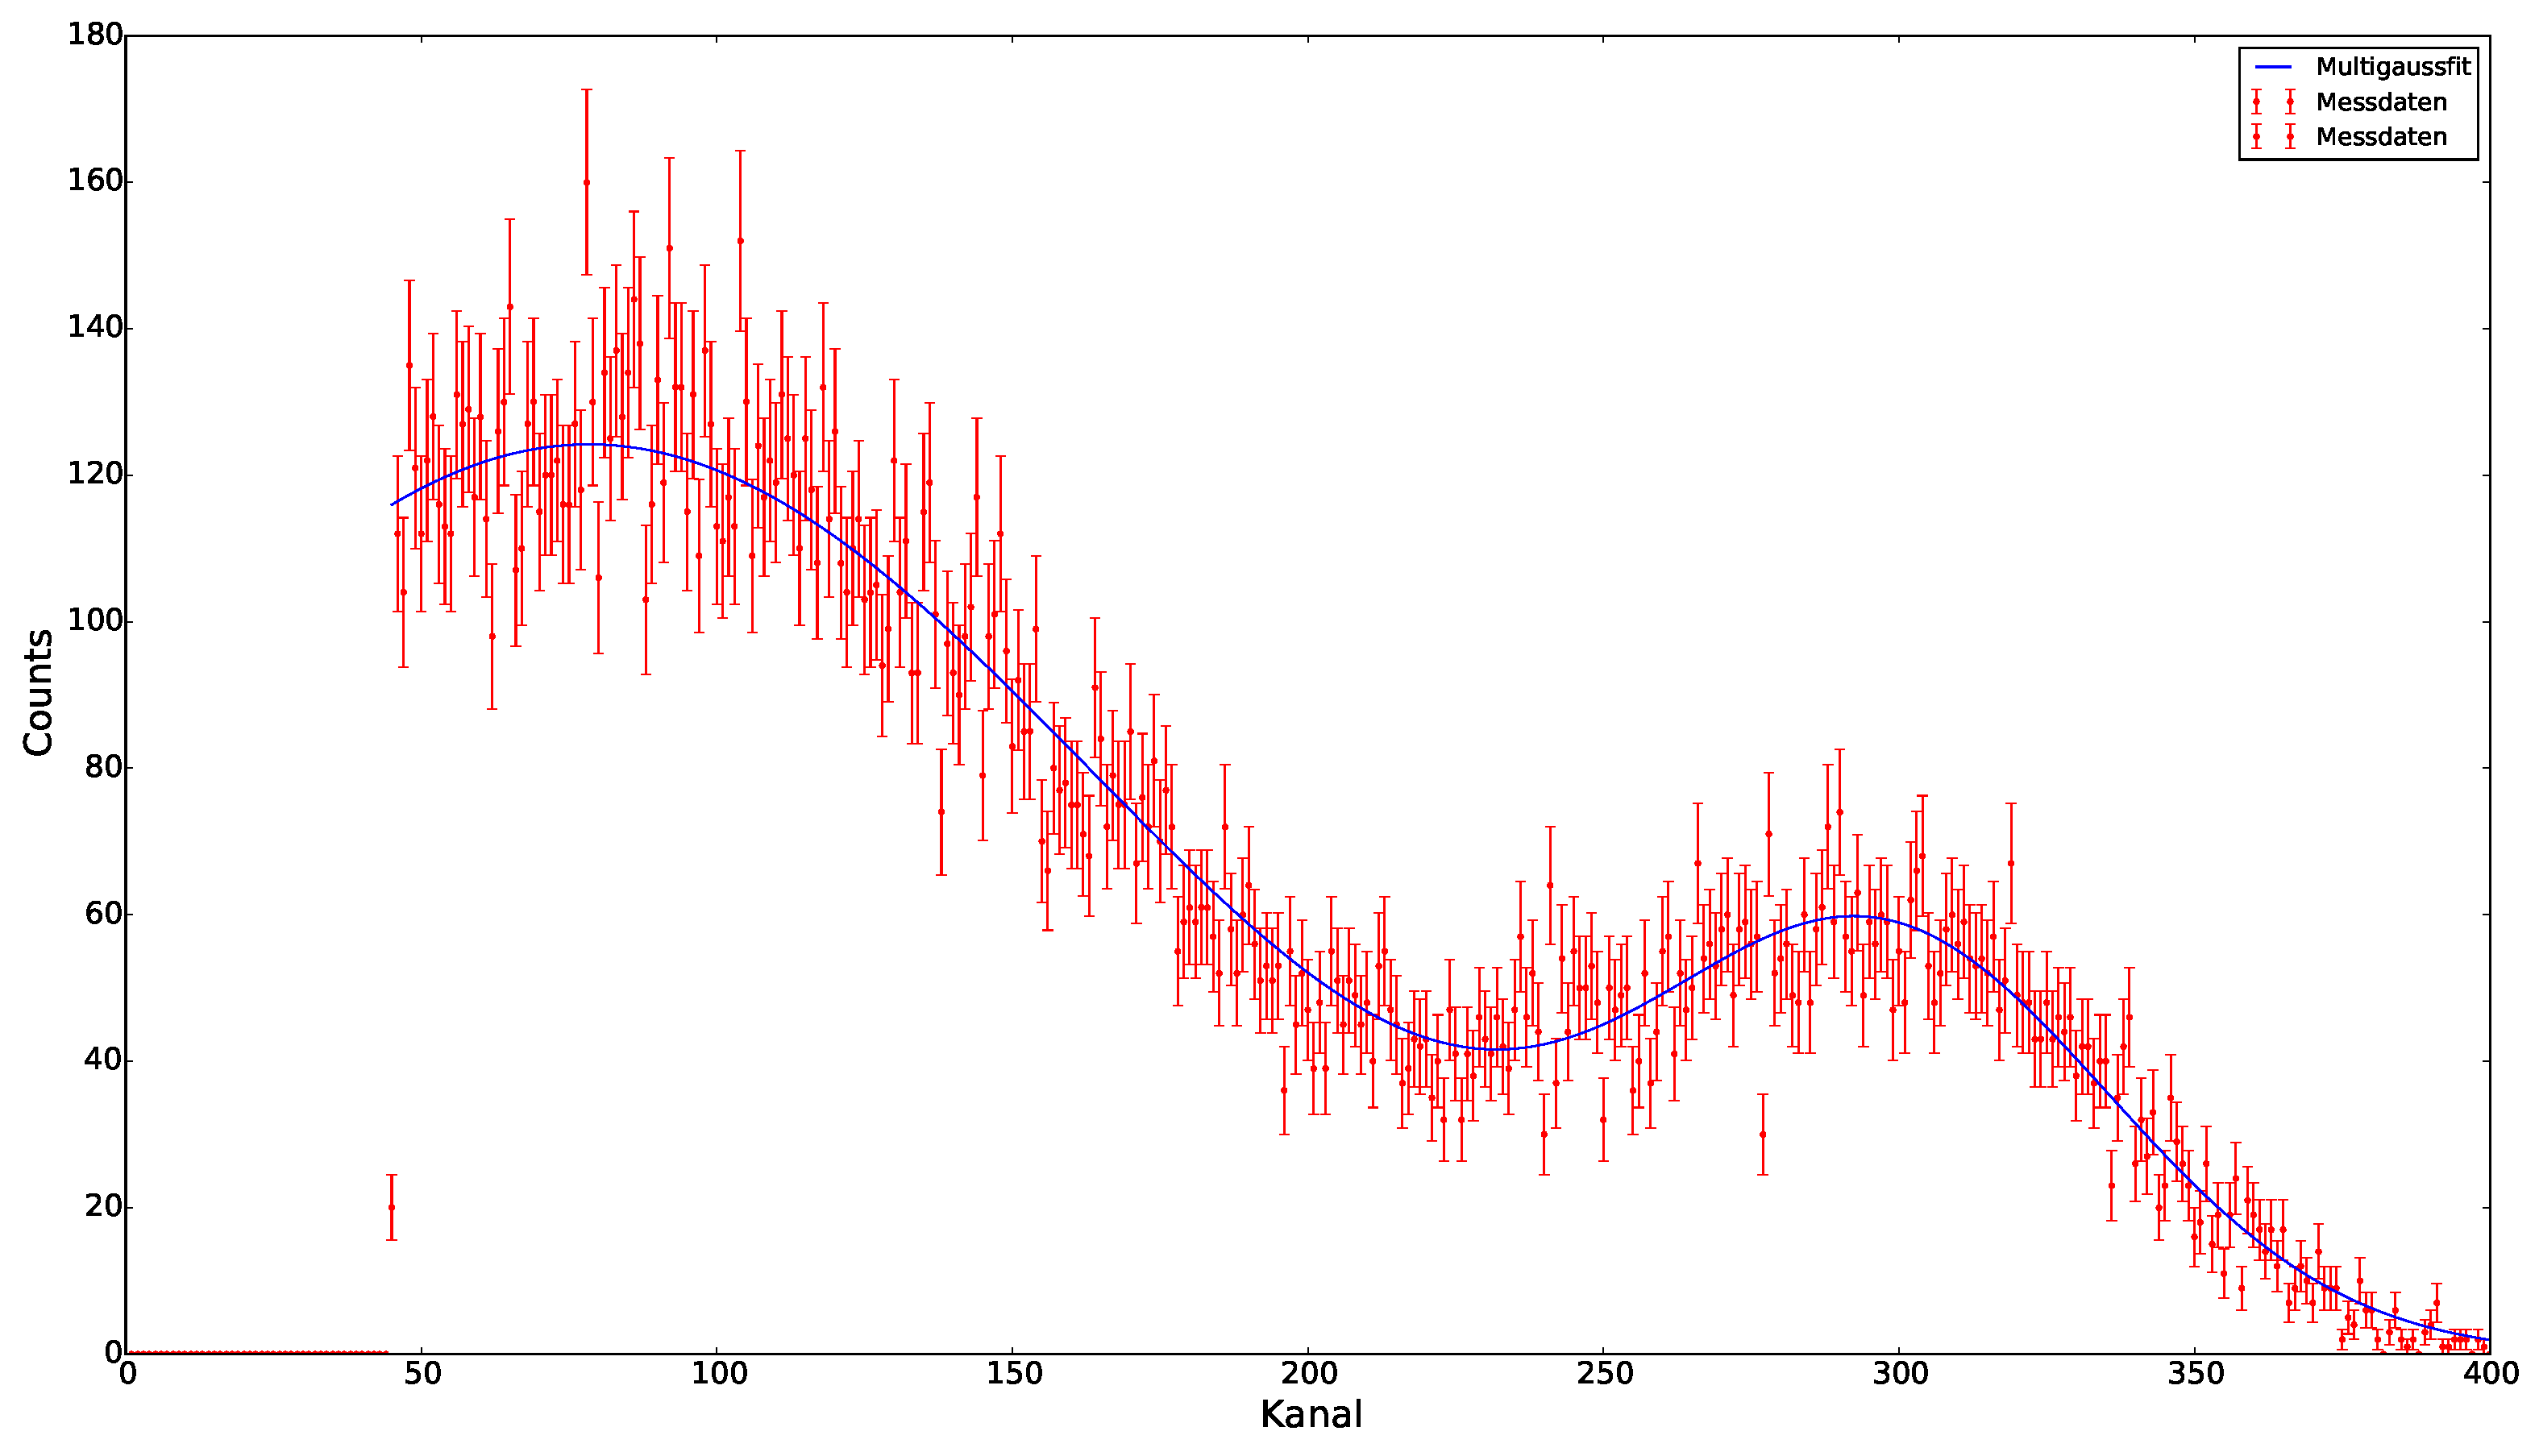
\includegraphics[scale=0.2]{ab_biebel.pdf}
	\caption{Schematischer Aufbau des Streukammer}
	\label{fig:ab_biebel}
\end{figure}


\section{Conclusion}
%im fazit nochmal alles zusammenfassen und den verlauf der messung absch�tzen
%gravierende sytematische probleme bei den messungen nochmal betonen und die wertigkeit unserer ergebnisse einordnen

In the first part of the experiment the 39 peaks of the nH$_3$ spectrum where measured and there relative absorption coefficients where calculated. In the second part the quadrupole moment where determined with a value of 5.02(9), with a deviation of 17.53\%. In the last part the broadening of the peaks according to the pressure was determined with 28 witch is a good measurement. 



\bibliography{ref}

\end{document}